% ------------------------------------------------------------------------------
% Este fichero es parte de la plantilla LaTeX para la realización de Proyectos
% Final de Grado, protegido bajo los términos de la licencia GFDL.
% Para más información, la licencia completa viene incluida en el
% fichero fdl-1.3.tex

% Copyright (C) 2012 SPI-FM. Universidad de Cádiz
% ------------------------------------------------------------------------------

En este capítulo estudiaremos la arquitectura general del sistema de información, el diseño de la interfaz de usuario, el diseño físico de datos y el diseño de componentes software.

\section{Diseño de la arquitectura}
\subsection{Arquitectura física}
Para estudiar la arquitectura nos debemos centrar en los componentes del servidor y en los componentes del cliente.\\
En el servidor debemos disponer de mysql para alojar la base de datos y de php 5.3 o superior ya que la versión de Symfony usada en la aplicación requiere la última versión de php. También disponer de un sistema para ejecutar trabajos programados en el servidor, para ello es recomendable que el servidor este sobre unix ya que dispondremos del servicio crontab.\\
En el cliente debemos disponer de una conexión a internet y un ordenador con cualquier sistema operativo y navegador.

\subsection{Arquitectura lógica}

Para la arquitectura lógica se determinó que la mejor manera de estructurar al sistema era haciendo uso del modelo-vista-controlador (MVC). En esta arquitectura se separan los datos y la lógica de negocio de la interfaz de usuario y el módulo de gestionar los eventos y las comunicaciones. Para ello se distinguen tres componentes:

\begin{itemize}
\item Modelo: Es la representación de la información que maneja la aplicación, es decir, es donde tenemos almacenados los datos. 

\item Vista: Es la representación gráfica que se muestra al usuario para que pueda ver la información o interactuar con ella.

\item Controlador: Es donde se recepcionan las peticiones del usuario e invoca al modelo cuando es necesario para almacenar o consultar información. Es el intermediario entre vista y modelo.
\end{itemize}

Aquí se muestra una imagen más detallada del proceso.

\begin{figure}[!htb]
  \centering
    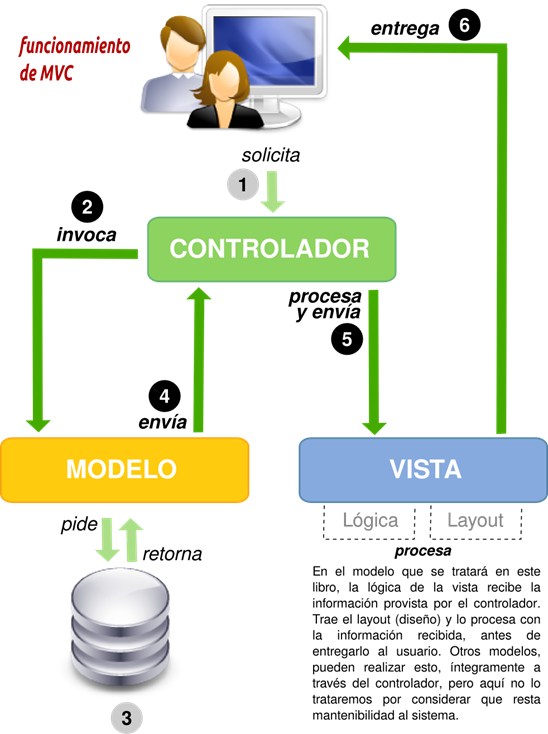
\includegraphics[scale=0.45]{mvc.png}
  \caption{Modelo-Vista-Controlador}
  \label{a}
\end{figure}

\section{Diseño de la interfaz de usuario} 

Para el diseño de la interfaz de usuario primero creamos unos prototipos y se le enseñaron al cliente al cual le parecieron correctos. Se pensó en un layout compuesto de tres zonas claramente diferenciadas: el header, content y footer.

\begin{figure}[!htb]
  \centering
    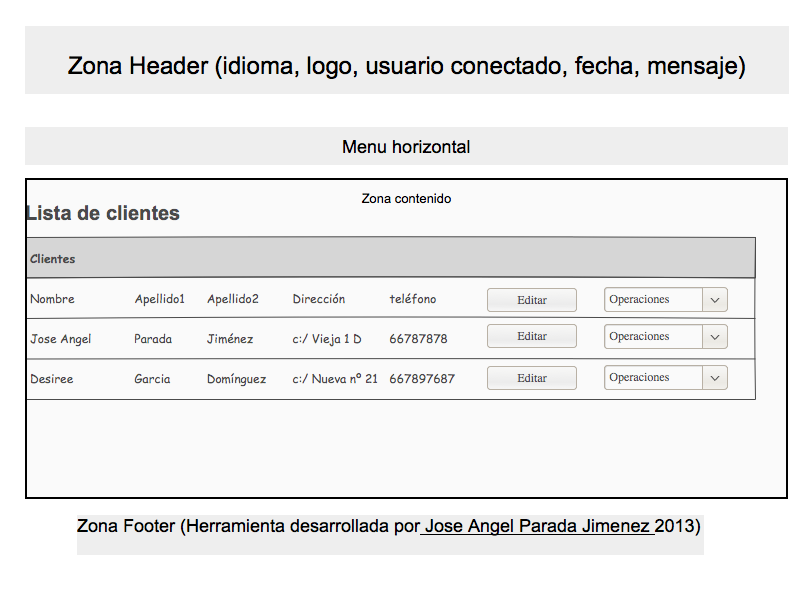
\includegraphics[scale=0.4]{mockup_cliente.png}
  \caption{Prototipo pantalla listar clientes}
  \label{a}
\end{figure}

\begin{figure}[!htb]
  \centering
    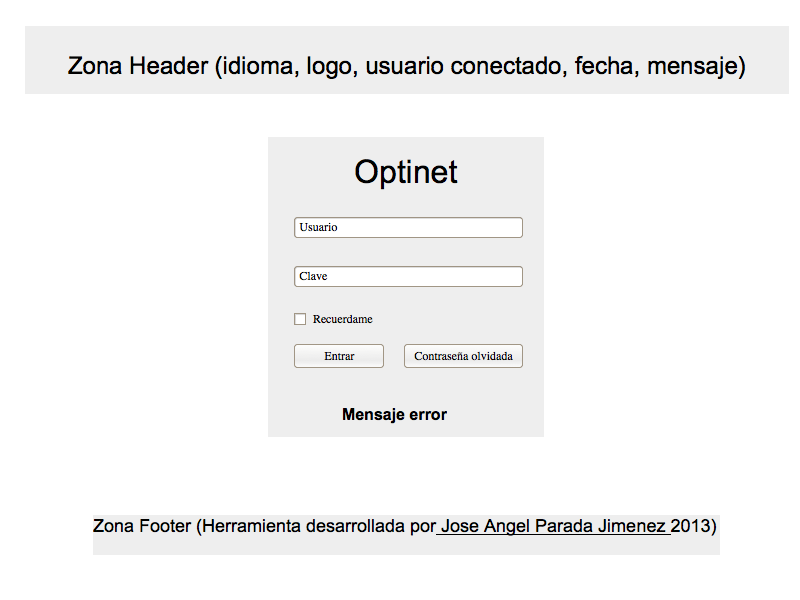
\includegraphics[scale=0.4]{mockup_login.png}
  \caption{Prototipo pantalla de login}
  \label{a}
\end{figure}

\newpage
\section{Diseño de datos}
En este apartado nos encontramos con el problema de diseñar la base de datos que pueda ser usada por nuestra aplicación web. Se estudiarán todos los apartados referentes al diseño del esquema conceptual: Se identificarán las clases, atributos, relaciones, restricciones adicionales y reglas de derivación necesarias.\\
La base de datos debe dar solución a todos los requisitos planteados anteriormente. La tarea en este momento es transformar el modelo conceptual realizado al modelo de datos en el que se apoyará nuestra aplicación para que funcione correctamente.\\
Para que todo funcione correctamente debemos garantizar la integridad de los datos que almacenamos en la base de datos. Para ello existen las condiciones de integridad de las bases de datos. Pueden ser de dos tipos:
\begin{itemize}

\item Reglas de integridad del usuario:
Son condiciones especificas que impone el creador de la base de datos para esa base de datos concreta.
\item Reglas de integridad del modelo:
Son condiciones de la teoría de las bases de datos que deben cumplir todas las bases de datos.
\begin{itemize}
\item Reglas de integridad de unicidad de clave primaria:
Ninguna tupla puede tener atributos repetidos en clave primaria.
\item Regla de integridad de clave primaria:
Los atributos primarios no pueden tener valores nulos.
\item Regla de integridad referencial:
No se deben tener claves foráneas sin correspondencia.
\item Regla de integridad de dominio:
Los valores de una tabla no pueden ser separados en dominios más simples.
\end{itemize}
\end{itemize}

Teniendo en cuenta estas restricciones de integridad, debemos conocer también como se relacionan las tablas de las bases de datos de acuerdo a su cardinalidad. 
\begin{itemize}
\item Relaciones 1:1\\
Se modifica cualquiera de las tablas que participan en la relación añadiendo la clave primaria de la otra.
\item Relaciones 1:N\\
Se modifica la tabla del lado muchos añadiendo la clave primaria de la otra.
\item Relaciones N:M\\
Se creá una nueva tabla añadiendo las claves primarias de las dos tablas y los atributos de la relación.
\item Relaciones de herencia\\
Se modifica la tabla añadiendo las claves primarias de la superclase.
\end{itemize}

A continuación detallamos el esquema relacional:\\
\begin{itemize}
\item \textbf{Tabla Cliente:}\\
Cliente (\underline{id},dni,nombre,apellido1,apellido2,direccion.localidad,provincia,telefono,movil,email)
\item\textbf{Tabla Producto:}\\
Producto (\underline{id},descripcion,stock,reservado,apartado,pventa,pcompra,iva,proveedor\_id,familia\_id)
\item\textbf{Tabla Familia:}\\
Familia(\underline{id},nombre)
\item \textbf{Tabla Proveedor:}\\
Proveedor(\underline{id},nombre,direccion,telefono,localidad,provincia,email)
\item \textbf{Tabla Role:}\\
Role (\underline{id},nombre) 
\item \textbf{Tabla Venta:}\\
Venta (\underline{id},total,pago,totalpago) 
\item \textbf{Tabla Reserva:}\\
Reserva (\underline{id},avisada,adelanto,apartado,total,pago,totalpago,venta\_id) 
\item \textbf{Tabla Devolución:}\\
Devolución (\underline{id},total,descripción,venta\_id)
 \item \textbf{Tabla Operación:}\\
Operación (\underline{id},fechaoper,tipo,cliente\_id,empleado\_id)
\item \textbf{Tabla Pedido:}\\
Pedido (\underline{id},fecha,fecharecepcion,total,recepciona\_id,empleado\_id,proveedor\_id)
\item \textbf{Tabla Modificacion:}\\
Modificación (\underline{id},fechamod,entidad,identificador,tipo,info,empleado\_id)
\item \textbf{Tabla Médico:}\\
Médico (\underline{id},titulacion,numero,color)
\item \textbf{Tabla Log:}\\
Log (\underline{id},fechalog,tipo,empleado\_id)
\item \textbf{Tabla Lineaspedido:}\\
Lineaspedido (\underline{pedido\_id},\underline{producto\_id},cantidad,precio,iva)
\item \textbf{Tabla Lineasoperación:}\\
Lineasoperación (\underline{operacion\_id},\underline{producto\_id},cantidad,precio,pcompra,iva,estado)
\item \textbf{Tabla Informe:}\\
Informe (\underline{id},fecha,odavsc,adavcc,adesf,adcil,adeje,adav,\\oiavsc,oiavcc,aiesf,oicil,oieje,oiav,problema,pupilar,worth,amsler,cita\_id)
\item \textbf{Tabla Festivo:}\\
Festivo (\underline{id},fecha)
\item \textbf{Tabla Empleado:}\\
Empleado (\underline{id},dni,nombre,username,apellido1,apellido2,email,localidad,provincia,claveusuario,\\telefono,movil,password,salt,direccion,fechaalta,activo,tipo,idioma,tema,role\_id)
\item \textbf{Tabla Cita:}\\
Cita (\underline{id},fechacita,medico\_id)
\item \textbf{Tabla Arqueo:}\\
Arqueo (\underline{id},fechaarqueo,efectivo,efectivocont,boletas,boletascont,estado,empleado\_id)
\item \textbf{Tabla Permiso:}\\
Permiso (\underline{id},fecha,inicio,fin,tipo,empleado\_id)
\end{itemize}
\newpage
\subsection{Normalización del modelo}
Llegado a este punto, solo nos queda iniciar el proceso de normalización ya que así evitaremos problemas de redundancias, ambigüedades, perdidas de información, etc.

\begin{itemize}
\item Primera forma normal:

Una relacion está en primera forma normal si para toda intersección de fila y columna tenemos un único valor. Es decir no pueden existir atributos compuestos.\\Las relaciones cumplen esta condición.

\item Segunda forma normal:

Una relación está en segunda forma normal si esta en primera y si los atributos que no forman parte de ninguna clave dependen de forma completa de la clave principal.\\Las relaciones cumplen esta condición.

\item Tercera forma normal:

Una relación está en tercera forma normal si esta en segunda y si no existe ninguna dependencia funcional transitiva entre los atributos que no son clave.\\Las relaciones cumplen esta condición.

\item Cuarta forma normal:

Una relación está en cuarta forma normal si para cada dependencia multivaluada no trivial viene determinada por una clave candidata.\\Las relaciones cumplen esta condición.

\item Quinta forma normal:

Una relación esta en quinta forma normal si esta en cuarta y cada relación de dependencia se encuentra definida por las claves candidatas.\\Las relaciones cumplen esta condición.
\end{itemize}


A continuación se detallan brevemente las entidades que intervienen en el sistema, comentando una descripción, el tipo, los atributos y el identificador.

\begin{table}
\centering  % used for centering table
\begin{tabular}{|c |c| c| c| c|c|} % centered columns (4 columns)
\hline\hline                        %inserts double horizontal lines
\multicolumn{6}{|>{\columncolor[gray]{0.93}}l|}{\textbf{Cliente: Almacena toda la información relativa a los clientes.}  } \\
\hline
\textbf{Atributo} & \textbf{Descripción} & \textbf{Tipo} & \textbf{Nulo} & \textbf{Pk} & \textbf{Fk}\\ [1ex] % inserts table 
%heading
\hline                  % inserts single horizontal line
Id & Identificador interno del objeto & INT & NO & SI & NO\\ % inserting body of the table
\hline
Dni & Documento nacional de identidad & VARCHAR(9) & NO & NO & NO\\ % inserting body of the table
\hline
Nombre & Nombre del cliente & VARCHAR(255) & NO & NO & NO\\
\hline
Apellido1 & Primer apellido del cliente & VARCHAR(255) & NO & NO & NO\\
\hline
Apellido2 & Segundo apellido del cliente & VARCHAR(255) & NO & NO & NO\\
\hline
Dirección & Dirección donde reside el cliente & VARCHAR(255)  & NO & NO & NO\\
\hline
Localidad & Localidad del cliente & VARCHAR(255)  & NO & NO & NO\\
\hline
Provincia & Provincia del cliente & VARCHAR(255)  & NO & NO & NO\\
\hline
Teléfono & Teléfono fijo del cliente & VARCHAR(9) & SI & NO & NO\\
\hline
Móvil & Teléfono móvil del cliente & VARCHAR(9)  & SI & NO & NO\\
\hline
Email & Dirección de correo del cliente & VARCHAR(255) & SI & NO & NO\\
\hline %inserts single line
\end{tabular}
\caption{Entidad:\textbf{ Cliente}} % title of Table
\end{table}


\begin{table}
\centering  % used for centering table
\begin{tabular}{|c |c| c| c| c|c |} % centered columns (4 columns)
\hline\hline                        %inserts double horizontal lines
\multicolumn{6}{|>{\columncolor[gray]{0.93}}l|}{\textbf{Proveedor: Almacena toda la información relativa a los proveedores.}  } \\
\hline
\textbf{Atributo} & \textbf{Descripción} & \textbf{Tipo} & \textbf{Nulo} & \textbf{Pk} & \textbf{Fk}\\ [1ex] % inserts table 
%heading
\hline                  % inserts single horizontal line
Id & Identificador interno del objeto & INT & NO & SI & NO \\ % inserting body of the table
\hline
Nombre & Nombre del proveedor & VARCHAR(255) & NO & NO & NO \\
\hline
Dirección & Dirección donde reside proveedor & VARCHAR(255)  & SI & NO & NO\\
\hline
Localidad & Localidad del proveedor & VARCHAR(255)  & SI & NO & NO\\
\hline
Provincia & Provincia del proveedor & VARCHAR(255)  & SI & NO & NO\\
\hline
Teléfono & Teléfono fijo del proveedor & VARCHAR(9) & SI & NO & NO\\
\hline
Email & Dirección de correo del proveedor & VARCHAR(255) & SI & NO & NO\\
\hline %inserts single line
\end{tabular}
\caption{Entidad:\textbf{ Proveedor}} % title of Table
\end{table}

\begin{table}
\centering  % used for centering table
\begin{tabular}{|c |c| c| c| c|c|} % centered columns (4 columns)
\hline\hline                        %inserts double horizontal lines
\multicolumn{6}{|>{\columncolor[gray]{0.93}}l|}{\textbf{Producto: Almacena toda la información relativa a los productos.}  } \\
\hline
\textbf{Atributo} & \textbf{Descripción} & \textbf{Tipo} & \textbf{Nulo} & \textbf{Pk} & \textbf{Fk}\\ [1ex] % inserts table 
%heading
\hline                  % inserts single horizontal line
Id & Identificador interno del objeto & INT & NO & SI & NO \\ % inserting body of the table
\hline
Descripción & Descripción general del producto & VARCHAR(255) & NO & NO & NO \\ % inserting body of the table
\hline
Pcompra & Precio al que se compra el producto & DOUBLE & NO & NO & NO \\ % inserting body of the table
\hline
Pventa & Precio de venta al público & DOUBLE & NO & NO & NO \\ % inserting body of the table
\hline
Stock & Stock del producto & INT & NO & NO & NO\\ % inserting body of the table
\hline
Reservado & Stock reservado del producto & INT & SI & NO & NO \\ % inserting body of the table
\hline
Apartado & Stock apartado del producto & INT & SI & NO & NO \\ % inserting body of the table
\hline
Iva & IVA del producto & INT & NO & NO & NO \\ % inserting body of the table
\hline
Proveedor\_id & Clave foránea & INT & SI & NO & SI\\ % inserting body of the table
\hline
Familia\_id & Clave foránea & INT & SI & NO & SI\\ % inserting body of the table
\hline
\end{tabular}
\caption{Entidad:\textbf{ Producto}} % title of Table
\end{table}


\begin{table}
\centering  % used for centering table
\begin{tabular}{|c |c| c| c| c|c|} % centered columns (4 columns)
\hline\hline                        %inserts double horizontal lines
\multicolumn{6}{|>{\columncolor[gray]{0.93}}l|}{\textbf{Empleado: Almacena toda la información relativa a los empleados.}  } \\
\hline
\textbf{Atributo} & \textbf{Descripción} & \textbf{Tipo} & \textbf{Nulo} & \textbf{Pk} & \textbf{Fk}\\ [1ex] % inserts table 
%heading
\hline                  % inserts single horizontal line
Id & Identificador interno del objeto & INT & NO & SI & NO \\ % inserting body of the table
\hline
Dni & Documento nacional de identidad & VARCHAR(9) & NO & NO & NO \\ % inserting body of the table
\hline
Nombre & Nombre del empleado & VARCHAR(255) & NO & NO & NO\\
\hline
Username & Nombre de usuario del empleado & VARCHAR(255) & NO & NO & NO\\
\hline
Apellido1 & Primer apellido del empleado & VARCHAR(255) & NO & NO & NO \\
\hline
Apellido2 & Segundo apellido del empleado & VARCHAR(255) & NO & NO & NO\\
\hline
Dirección & Dirección donde reside el empleado & VARCHAR(255)  & NO & NO & NO\\
\hline
Localidad & Localidad del empleado & VARCHAR(255)  & NO & NO & NO\\
\hline
Provincia & Provincia del empleado & VARCHAR(255)  & NO & NO & NO\\
\hline
Teléfono & Teléfono fijo del empleado & VARCHAR(9) & SI & NO & NO\\
\hline
Móvil & Teléfono móvil del empleado & VARCHAR(9)  & SI & NO & NO\\
\hline
Email & Dirección de correo del empleado & VARCHAR(255) & NO & NO & NO\\
\hline
Password & Contraseña cifrada del empleado & VARCHAR(255) & NO & NO & NO\\
\hline
Salt & Semilla para el password del empleado & VARCHAR(255) & NO & NO & NO\\
\hline
Claveusuario & Clave para generar nueva contraseña & VARCHAR(255) & NO & NO & NO\\
\hline
Fechaalta & Fecha de creación del empleado & DATETIME & NO & NO & NO\\
\hline
Idioma & Idioma elegido por el empleado & VARCHAR(7) & NO & NO & NO\\
\hline
Tema & Tema elegido por el empleado & VARCHAR(10) & NO & NO & NO\\
\hline
Tipo & Tipo de empleado & INT & NO & NO & NO\\
\hline
Activo & Indica si el empleado está activo & INT & NO & NO & NO\\
\hline
Role\_id & Clave foránea & INT & SI & NO & SI\\
\hline
\end{tabular}
\caption{Entidad:\textbf{ Empleado}} % title of Table
\end{table}


\begin{table}
\centering  % used for centering table
\begin{tabular}{|c |c| c| c| c|c|} % centered columns (4 columns)
\hline\hline                        %inserts double horizontal lines
\multicolumn{6}{|>{\columncolor[gray]{0.93}}l|}{\textbf{Médico: Almacena información especifica del empleado médico.}  } \\
\hline
\textbf{Atributo} & \textbf{Descripción} & \textbf{Tipo} & \textbf{Nulo} & \textbf{Pk} &\textbf{Fk}\\ [1ex] % inserts table 
%heading
\hline                  % inserts single horizontal line
Id & Identificador interno del objeto & INT & NO & SI & NO\\ % inserting body of the table
\hline                  % inserts single horizontal line
Titulación & Titulación del médico & VARCHAR(225) & SI & NO & NO\\ % inserting body of the table
\hline
Número & Número de colegiado & VARCHAR(255) & SI & NO & NO\\ % inserting body of the table
\hline
Color & Color del médico & VARCHAR(255) & NO & NO & NO\\ % inserting body of the table
\hline
\end{tabular}
\caption{Entidad:\textbf{ Médico}} % title of Table
\end{table}

\begin{table}
\centering  % used for centering table
\begin{tabular}{|c |c| c| c| c|c|} % centered columns (4 columns)
\hline\hline                        %inserts double horizontal lines
\multicolumn{6}{|>{\columncolor[gray]{0.93}}l|}{\textbf{Modificación: Almacena las modificaciones en el sistema que hacen los empleados.}  } \\
\hline
\textbf{Atributo} & \textbf{Descripción} & \textbf{Tipo} & \textbf{Nulo} & \textbf{Pk} & \textbf{Fk}\\ [1ex] % inserts table 
%heading
\hline                  % inserts single horizontal line
Id & Identificador interno del objeto & INT & NO & SI & NO \\ % inserting body of the table
\hline
Fechamod & Fecha creación de la modificación & DATETIME & NO & NO & NO \\ % inserting body of the table
\hline
Tipo & Tipo de modificación & VARCHAR(255) & SI & NO & NO\\ % inserting body of the table
\hline
Entidad & Entidad que se ha modificado & VARCHAR(255) & SI & NO & NO \\ % inserting body of the table
\hline
Identificador & Identificador del objeto modificado & VARCHAR(255) & SI & NO & NO \\ % inserting body of the table
\hline
Info & Información de los cambios realizados & VARCHAR(255) & SI & NO & NO \\ % inserting body of the table
\hline
Empleado\_id & Clave foránea & INT & SI & NO & SI \\ % inserting body of the table
\hline
\end{tabular}
\caption{Entidad:\textbf{ Modificación}} % title of Table
\end{table}


\begin{table}
\centering  % used for centering table
\begin{tabular}{|c |c| c| c| c| c|} % centered columns (4 columns)
\hline\hline                        %inserts double horizontal lines
\multicolumn{6}{|>{\columncolor[gray]{0.93}}l|}{\textbf{Log: Almacena cuando entran y salen los empleados del sistema.}  } \\
\hline
\textbf{Atributo} & \textbf{Descripción} & \textbf{Tipo} & \textbf{Nulo} & \textbf{Pk} & \textbf{Fk}\\ [1ex] % inserts table 
%heading
\hline                  % inserts single horizontal line
Id & Identificador interno del objeto & INT & NO & SI & NO \\ % inserting body of the table
\hline
Fechalog & Fecha realización de la operación & DATETIME & NO & NO & NO\\ % inserting body of the table
\hline
Tipo & Información entrada o salida & VARCHAR(255) & SI & NO & NO \\ % inserting body of the table
\hline
Empleado\_id & Clave foránea & INT & SI & NO & SI \\ % inserting body of the table
\hline
\end{tabular}
\caption{Entidad:\textbf{ Log}} % title of Table
\end{table}


\begin{table}
\centering  % used for centering table
\begin{tabular}{|c |c| c| c| c| c|} % centered columns (4 columns)
\hline\hline                        %inserts double horizontal lines
\multicolumn{6}{|>{\columncolor[gray]{0.93}}l|}{\textbf{Rol: Almacena los distintos roles que pueden tener los empleados.}  } \\
\hline
\textbf{Atributo} & \textbf{Descripción} & \textbf{Tipo} & \textbf{Nulo} & \textbf{Pk} & \textbf{Fk}\\ [1ex] % inserts table 
%heading
\hline                  % inserts single horizontal line
Id & Identificador interno del objeto & INT & NO & SI & NO \\ % inserting body of the table
\hline
Nombre & Nombre del rol & VARCHAR(255) & NO & NO & NO \\ % inserting body of the table
\hline
\end{tabular}
\caption{Entidad:\textbf{ Rol}} % title of Table
\end{table}


\begin{table}
\centering  % used for centering table
\begin{tabular}{|c |c| c| c| c|c|} % centered columns (4 columns)
\hline\hline                        %inserts double horizontal lines
\multicolumn{6}{|>{\columncolor[gray]{0.93}}l|}{\textbf{Familia: Almacena las familias que existen para poder organizar los productos.}  } \\
\hline
\textbf{Atributo} & \textbf{Descripción} & \textbf{Tipo} & \textbf{Nulo} & \textbf{Pk} & \textbf{Fk}\\ [1ex] % inserts table 
%heading
\hline                  % inserts single horizontal line
Id & Identificador interno del objeto & INT & NO & SI & NO \\ % inserting body of the table
\hline
Nombre & Nombre de la familia & VARCHAR(255) & NO & NO & NO \\ % inserting body of the table
\hline
\end{tabular}
\caption{Entidad:\textbf{ Familia}} % title of Table
\end{table}


\begin{table}
\centering  % used for centering table
\begin{tabular}{|c |c| c| c| c| c|} % centered columns (4 columns)
\hline\hline                        %inserts double horizontal lines
\multicolumn{6}{|>{\columncolor[gray]{0.93}}l|}{\textbf{Informe: Almacena toda la información de los informes que realizan los medicos.}  } \\
\hline
\textbf{Atributo} & \textbf{Descripción} & \textbf{Tipo} & \textbf{Nulo} & \textbf{Pk} & \textbf{Fk}\\ [1ex] % inserts table 
%heading
\hline                  % inserts single horizontal line
Id & Identificador interno del objeto & INT & NO & SI & NO\\ % inserting body of the table
\hline
Fecha & Fecha realización informe & DATETIME & NO & NO & NO \\ % inserting body of the table
\hline
Odavsc & Ojo derecho odavsc & VARCHAR(255) & SI & NO & NO \\ % inserting body of the table
\hline
Odavcc & Ojo derecho odacc & VARCHAR(255) & SI & NO & NO\\ % inserting body of the table
\hline
Odesf & Esfera del ojo derecho & VARCHAR(255) & SI & NO & NO \\ % inserting body of the table
\hline
Odcil & Cilindro del ojo derecho & VARCHAR(255) & SI & NO & NO\\ % inserting body of the table
\hline
Odeje & Eje del ojo derecho & VARCHAR(255) & SI & NO & NO\\ % inserting body of the table
\hline
Odav & Ojo derecho odav & VARCHAR(255) & SI & NO & NO \\ % inserting body of the table
\hline
Oiavsc & Ojo izquierdo oiavsc & VARCHAR(255) & SI & NO & NO\\ % inserting body of the table
\hline
Oiavcc & Ojo izquierdo oiacc & VARCHAR(255) & SI & NO & NO\\ % inserting body of the table
\hline
Oiesf & Esfera del ojo izquierdo & VARCHAR(255) & SI & NO & NO \\ % inserting body of the table
\hline
Oicil & Cilindro del ojo izquierdo & VARCHAR(255) & SI & NO & NO \\ % inserting body of the table
\hline
Oieje & Eje del ojo izquierdo & VARCHAR(255) & SI & NO &NO \\ % inserting body of the table
\hline
Problema & Problema de la visión & VARCHAR(255) & NO & NO & NO \\ % inserting body of the table
\hline
Pupilar & Reacción pupilar & VARCHAR(255) & NO & NO  & NO\\ % inserting body of the table
\hline
Worth & Test de Worth & VARCHAR(255) & NO & NO & NO \\ % inserting body of the table
\hline
Amsler & Rejilla de Amsler & VARCHAR(255) & NO & NO & NO \\ % inserting body of the table
\hline
Cita\_id & Clave foránea & INT & SI & NO & SI \\ % inserting body of the table
\hline
\end{tabular}
\caption{Entidad:\textbf{ Informe}} % title of Table
\end{table}


\begin{table}
\centering  % used for centering table
\begin{tabular}{|c |c| c| c| c| c|} % centered columns (4 columns)
\hline\hline                        %inserts double horizontal lines
\multicolumn{6}{|>{\columncolor[gray]{0.93}}l|}{\textbf{Operación: Almacena las distintas operaciones que puede realizar el empleado}  } \\
\hline
\textbf{Atributo} & \textbf{Descripción} & \textbf{Tipo} & \textbf{Nulo} & \textbf{Pk} & \textbf{Fk}\\ [1ex] % inserts table 
%heading
\hline                  % inserts single horizontal line
Id & Identificador interno del objeto & INT & NO & SI & NO\\ % inserting body of the table
\hline
Fechaoper & Fecha realización de la operación & DATETIME & NO & NO & NO \\ % inserting body of the table
\hline
Tipo & Tipo de operación & VARCHAR(255) & NO & NO & NO \\ % inserting body of the table
\hline
Cliente\_id & Clave foránea & INT & SI & NO & SI \\ % inserting body of the table
\hline
Empleado\_id & Clave foránea & INT & SI & NO & SI \\ % inserting body of the table
\hline
\end{tabular}
\caption{Entidad:\textbf{ Operación}} % title of Table
\end{table}


\begin{table}
\centering  % used for centering table
\begin{tabular}{|c |c| c| c| c| c|} % centered columns (4 columns)
\hline\hline                        %inserts double horizontal lines
\multicolumn{6}{|>{\columncolor[gray]{0.93}}l|}{\textbf{Cita: Almacena toda la información relativa a las citas.}  } \\
\hline
\textbf{Atributo} & \textbf{Descripción} & \textbf{Tipo} & \textbf{Nulo} & \textbf{Pk} & \textbf{Fk}\\ [1ex] % inserts table 
%heading
\hline                  % inserts single horizontal line
Id & Identificador interno del objeto & INT & NO & NO & NO \\ % inserting body of the table
\hline
Fechacita & Fecha realización de la cita & DATETIME & NO & NO & NO\\ % inserting body of the table
\hline
Medico\_id & Clave foránea & INT & SI & NO & SI\\ % inserting body of the table
\hline
\end{tabular}
\caption{Entidad:\textbf{ Cita}} % title of Table
\end{table}

\begin{table}
\centering  % used for centering table
\begin{tabular}{|c |c| c| c| c|c|} % centered columns (4 columns)
\hline\hline                        %inserts double horizontal lines
\multicolumn{6}{|>{\columncolor[gray]{0.93}}l|}{\textbf{Venta: Almacena toda la información relativa a las ventas.}  } \\
\hline
\textbf{Atributo} & \textbf{Descripción} & \textbf{Tipo} & \textbf{Nulo} & \textbf{Pk} & \textbf{Fk}\\ [1ex] % inserts table 
%heading
\hline                  % inserts single horizontal line
Id & Identificador interno del objeto & INT & NO & SI & NO \\ % inserting body of the table
\hline
Total & Importe total de la venta & DOUBLE & NO & NO & NO \\ % inserting body of the table
\hline
Pago & Forma de pago de la venta & VARCHAR(255) & NO & NO & NO \\ % inserting body of the table
\hline
Totalpago & Importe entregado por el cliente & DOUBLE & SI & NO & NO \\ % inserting body of the table
\hline
\end{tabular}
\caption{Entidad:\textbf{ Venta}} % title of Table
\end{table}

\begin{table}
\centering  % used for centering table
\begin{tabular}{|c |c| c| c| c| c|} % centered columns (4 columns)
\hline\hline                        %inserts double horizontal lines
\multicolumn{6}{|>{\columncolor[gray]{0.93}}l|}{\textbf{Reserva: Almacena toda la información relativa a las reservas.}  } \\
\hline
\textbf{Atributo} & \textbf{Descripción} & \textbf{Tipo} & \textbf{Nulo} & \textbf{Pk} & \textbf{Fk}\\ [1ex] % inserts table 
%heading
\hline                  % inserts single horizontal line
Id & Identificador interno del objeto & INT & NO & NO & NO \\ % inserting body of the table
\hline
Total & Importe total de la reserva & DOUBLE & NO & NO  & NO\\ % inserting body of the table
\hline
Adelanto & Importe adelantado reserva & DOUBLE & NO & NO & NO \\ % inserting body of the table
\hline
Avisada & Indicación si la reserva está avisada & DATETIME & SI & NO & NO \\ % inserting body of the table
\hline
Pago & Forma de pago de la reserva & VARCHAR(255) & NO & NO & NO \\ % inserting body of the table
\hline
Totalpago & Importe entregado por el cliente & DOUBLE & SI & NO & NO \\ % inserting body of the table
\hline
Venta\_id & Clave foránea & INT & SI & NO & SI \\ % inserting body of the table
\hline
\end{tabular}
\caption{Entidad:\textbf{ Reserva}} % title of Table
\end{table}

\begin{table}
\centering  % used for centering table
\begin{tabular}{|c |c| c| c| c|c|} % centered columns (4 columns)
\hline\hline                        %inserts double horizontal lines
\multicolumn{6}{|>{\columncolor[gray]{0.93}}l|}{\textbf{Devolución: Almacena toda la información relativa a las devoluciones.}  } \\
\hline
\textbf{Atributo} & \textbf{Descripción} & \textbf{Tipo} & \textbf{Nulo} & \textbf{Pk} & \textbf{Fk}\\ [1ex] % inserts table 
%heading
\hline                  % inserts single horizontal line
Id & Identificador interno del objeto & INT & NO & NO & NO \\ % inserting body of the table
\hline
Total & Importe total de la devolución & DOUBLE & NO & NO & NO \\ % inserting body of the table
\hline
Descripción& Descripción de la devolución & VARCHAR(255) & SI & NO & NO\\ % inserting body of the table
\hline
Venta\_id & Clave foránea & INT & SI & NO & SI \\ % inserting body of the table
\hline
\end{tabular}
\caption{Entidad:\textbf{ Devolución}} % title of Table
\end{table}


\begin{table}
\centering  % used for centering table
\begin{tabular}{|c |c| c| c| c| c|} % centered columns (4 columns)
\hline\hline                        %inserts double horizontal lines
\multicolumn{6}{|>{\columncolor[gray]{0.93}}l|}{\textbf{Pedido: Almacena toda la información relativa a los pedidos.}  } \\
\hline
\textbf{Atributo} & \textbf{Descripción} & \textbf{Tipo} & \textbf{Nulo} & \textbf{Pk} & \textbf{Fk}\\ [1ex] % inserts table 
%heading
\hline                  % inserts single horizontal line
Id & Identificador interno del objeto & INT & NO & SI & NO \\ % inserting body of the table
\hline
Fecha & Fecha realización del pedido & DATETIME & NO & NO & NO\\ % inserting body of the table
\hline
Fecharecepción & Fecha recepción del pedido & DATETIME & NO & NO & NO \\ % inserting body of the table
\hline
Total & Importe total del pedido & DOUBLE & NO & NO & NO\\ % inserting body of the table
\hline
Recepciona\_id & Clave foránea & INT & SI & NO & NO\\ % inserting body of the table
\hline
Empleado\_id & Clave foránea & INT & SI & NO & NO\\ % inserting body of the table
\hline
Proveedor\_id & Clave foránea & INT & SI & NO & NO\\ % inserting body of the table
\hline
\end{tabular}
\caption{Entidad:\textbf{ Pedido}} % title of Table
\end{table}

\begin{table}
\centering  % used for centering table
\begin{tabular}{|c |c| c| c| c| c|} % centered columns (4 columns)
\hline\hline                        %inserts double horizontal lines
\multicolumn{6}{|>{\columncolor[gray]{0.93}}l|}{\textbf{Linea Operacion: Se deben modificar productos sin que afecte a las operaciones.}  } \\
\hline
\textbf{Atributo} & \textbf{Descripción} & \textbf{Tipo} & \textbf{Nulo} & \textbf{Pk} & \textbf{Fk}\\ [1ex] % inserts table 
%heading
\hline                  % inserts single horizontal line
Operacion\_id & Identificador interno del objeto & INT & NO & SI & SI \\ % inserting body of the table
\hline
Producto\_id & Identificador interno del objeto & INT & NO & SI & SI \\ % inserting body of the table
\hline
Cantidad & Cantidad del producto & INT & NO & NO & NO \\ % inserting body of the table
\hline
Precio & Precio producto en ese instante & DOUBLE & NO & NO & NO\\ % inserting body of the table
\hline
Pcompra & Precio de compra en ese instante & DOUBLE & NO & NO & NO\\ % inserting body of the table
\hline
Iva & Iva del producto en ese instante & INT & NO & NO & NO\\ % inserting body of the table
\hline
Estado & Estado del producto para devoluciones & VARCHAR(255) & SI & NO & NO\\ % inserting body of the table
\hline
\end{tabular}
\caption{Entidad:\textbf{ Linea Operación}} % title of Table
\end{table}

\begin{table}
\centering  % used for centering table
\begin{tabular}{|c |c| c| c| c| c|} % centered columns (4 columns)
\hline\hline                        %inserts double horizontal lines
\multicolumn{6}{|>{\columncolor[gray]{0.93}}l|}{\textbf{Linea Pedido: Se deben modificar productos sin que afecte a las operaciones.}  } \\
\hline
\textbf{Atributo} & \textbf{Descripción} & \textbf{Tipo} & \textbf{Nulo} & \textbf{Pk} & \textbf{Fk}\\ [1ex] % inserts table 
%heading
\hline                  % inserts single horizontal line
Pedido\_id & Identificador interno del objeto & INT & NO & SI & SI \\ % inserting body of the table
\hline
Producto\_id & Identificador interno del objeto & INT & NO & SI & SI \\ % inserting body of the table
\hline
Cantidad & Cantidad del producto & INT & NO & NO & NO \\ % inserting body of the table
\hline
Precio & Precio producto en ese instante & DOUBLE & NO & NO & NO\\ % inserting body of the table
\hline
Iva & Iva producto en ese instante & INT & NO & NO & NO\\ % inserting body of the table
\hline
\end{tabular}
\caption{Entidad:\textbf{ Linea Pedido}} % title of Table
\end{table}


\clearpage

\begin{table}
\centering  % used for centering table
\begin{tabular}{|c |c| c| c| c| c|} % centered columns (4 columns)
\hline\hline                        %inserts double horizontal lines
\multicolumn{6}{|>{\columncolor[gray]{0.93}}l|}{\textbf{Festivo: Almacena la información relativa a los dias festivos.}  } \\
\hline
\textbf{Atributo} & \textbf{Descripción} & \textbf{Tipo} & \textbf{Nulo} & \textbf{Pk} & \textbf{Fk}\\ [1ex] % inserts table 
%heading
\hline                  % inserts single horizontal line
Id & Identificador interno del objeto & INT & NO & SI & NO \\ % inserting body of the table
\hline
Fecha & Fecha del dia festivo & DATETIME & NO & NO & NO \\ % inserting body of the table
\hline
\end{tabular}
\caption{Entidad:\textbf{ Festivo}} % title of Table
\end{table}


\begin{table}
\centering  % used for centering table
\begin{tabular}{|c |c| c| c| c| c|} % centered columns (4 columns)
\hline\hline                        %inserts double horizontal lines
\multicolumn{6}{|>{\columncolor[gray]{0.93}}l|}{\textbf{Arqueo: Almacena la información relativa a los arqueos.}  } \\
\hline
\textbf{Atributo} & \textbf{Descripción} & \textbf{Tipo} & \textbf{Nulo} & \textbf{Pk} & \textbf{Fk}\\ [1ex] % inserts table 
%heading
\hline                  % inserts single horizontal line
Id & Identificador interno del objeto & INT & NO & SI & NO \\ % inserting body of the table
\hline
Fechaarqueo & Fecha realización arqueo & DATETIME & NO & NO & NO \\ % inserting body of the table
\hline
Efectivo & Dinero en efectivo del sistema & DOUBLE & NO & NO & NO \\ % inserting body of the table
\hline
Efectivocont & Dinero en efectivo contado & DOUBLE & NO & NO & NO \\ % inserting body of the table
\hline
Boletas & Boletas del sistema & INT & NO & NO & NO \\ % inserting body of the table
\hline
Boletascont & Boletas contadas & INT & NO & NO & NO \\ % inserting body of the table
\hline
Estado & Estado del arqueo & BOOL & NO & NO & NO \\ % inserting body of the table
\hline
Empleado\_id & Clave foránea & INT & SI & NO & NO\\ % inserting body of the table
\hline
\end{tabular}
\caption{Entidad:\textbf{ Arqueo}} % title of Table
\end{table}

\begin{table}
\centering  % used for centering table
\begin{tabular}{|c |c| c| c| c| c|} % centered columns (4 columns)
\hline\hline                        %inserts double horizontal lines
\multicolumn{6}{|>{\columncolor[gray]{0.93}}l|}{\textbf{Permiso: Almacena la información relativa a los permisos de los usuarios.}  } \\
\hline
\textbf{Atributo} & \textbf{Descripción} & \textbf{Tipo} & \textbf{Nulo} & \textbf{Pk} & \textbf{Fk}\\ [1ex] % inserts table 
%heading
\hline                  % inserts single horizontal line
Id & Identificador interno del objeto & INT & NO & SI & NO \\ % inserting body of the table
\hline
Fecha & Fecha realización permiso & DATETIME & NO & NO & NO \\ % inserting body of the table
\hline
Inicio & Fecha de inicio del permiso & DATETIME & NO & NO & NO \\ % inserting body of the table
\hline
Fin & Fecha de fin del permiso & DATETIME & NO & NO & NO \\ % inserting body of the table
\hline
Tipo & Tipo de permiso & VARCHAR(255) & NO & NO & NO \\ % inserting body of the table
\hline
Empleado\_id & Clave foránea & INT & SI & NO & NO\\ % inserting body of the table
\hline
\end{tabular}
\caption{Entidad:\textbf{ Permiso}} % title of Table
\end{table}

\clearpage

En este apartado estudiaremos los distintos tipos de relaciones que existen:\\
\begin{table}[htb]  % used for centering table
\centering  % used for centering table
\begin{tabular}{|l |l| l|} % centered columns (4 columns)
\hline\hline                        %inserts double horizontal lines
\multicolumn{3}{|>{\columncolor[gray]{0.93}}l|}{\textbf{Descripción de los distintos tipos de relaciones}  } \\
\hline
\textbf{Tipo} & \textbf{Descripción} & \textbf{Entidades}\\ [1ex] % inserts table 
%heading
\hline                  % inserts single horizontal line
Realiza & Un cliente realiza una operación & Cliente - Operación \\ % inserting body of the table
\hline
Se compone de & Una operación se compone de lineas de operación & Operación - Linea Operación  \\ % inserting body of the table
\hline
Contiene & Una linea operación contiene un produto & Linea Operación - Producto  \\ % inserting body of the table
\hline
Pertenece & Un producto pertenece a una familia & Producto - Familia  \\ % inserting body of the table
\hline
Contiene & Una linea de pedido contiene un producto & Linea Pedido - Producto  \\ % inserting body of the table
\hline
Compuesto de & Un pedido se compone de lineas de pedido & Pedido - Linea Pedido  \\ % inserting body of the table
\hline
Realizado a & Un pedido se realiza a un proveedor & Pedido - Proveedor  \\ % inserting body of the table
\hline
Hace & Un empleado hace pedidos & Empleado - Pedido  \\ % inserting body of the table
\hline
Recepciona & Un empleado recepciona pedidos & Empleado - Pedido  \\ % inserting body of the table
\hline
Suministra & Un proveedor suministra productos & Proveedor - Producto  \\ % inserting body of the table
\hline
Hace & Un empleado hace modificaciones & Empleado - Modificación  \\ % inserting body of the table
\hline
Tiene & Un empleado tiene un log & Empleado - Log  \\ % inserting body of the table
\hline
Tiene & Un empleado tiene un rol & Empleado - Rol  \\ % inserting body of the table
\hline
Dirige & Un empleado dirige operaciones & Empleado - Operación  \\ % inserting body of the table
\hline
Acude & Un médico acude a una cita & Médico - Cita  \\ % inserting body of the table
\hline
Tiene & Un empleado tiene permisos & Empleado - Permiso  \\ % inserting body of the table
\hline
Hace & Un empleado hace arqueos & Empleado - Arqueo  \\ % inserting body of the table
\hline
Pertenece & Un informe pertenece a una cita & Cita - Informe  \\ % inserting body of the table
\hline
Se convierte & Una reserva se convierte en una venta & Reserva - Venta  \\ % inserting body of the table
\hline
Pertenece & Una devolución pertenece a una venta & Devolución - Venta  \\ % inserting body of the table
\hline
\end{tabular}
\caption{Descripción de los tipos de relaciones} % title of Table
\end{table}

\clearpage
\newpage
\section{Diseño de componentes}
\subsection{Diagrama de clases de diseño}
Se han omitido las clases controlador y vista de productos, proveedores, familias puesto que siguen un comportamiento similar.
Para poder construir el diagrama, se ha tenido que dividir en dos diagramas que se muestran a continuación:

\begin{figure}[!htb]
  \centering
    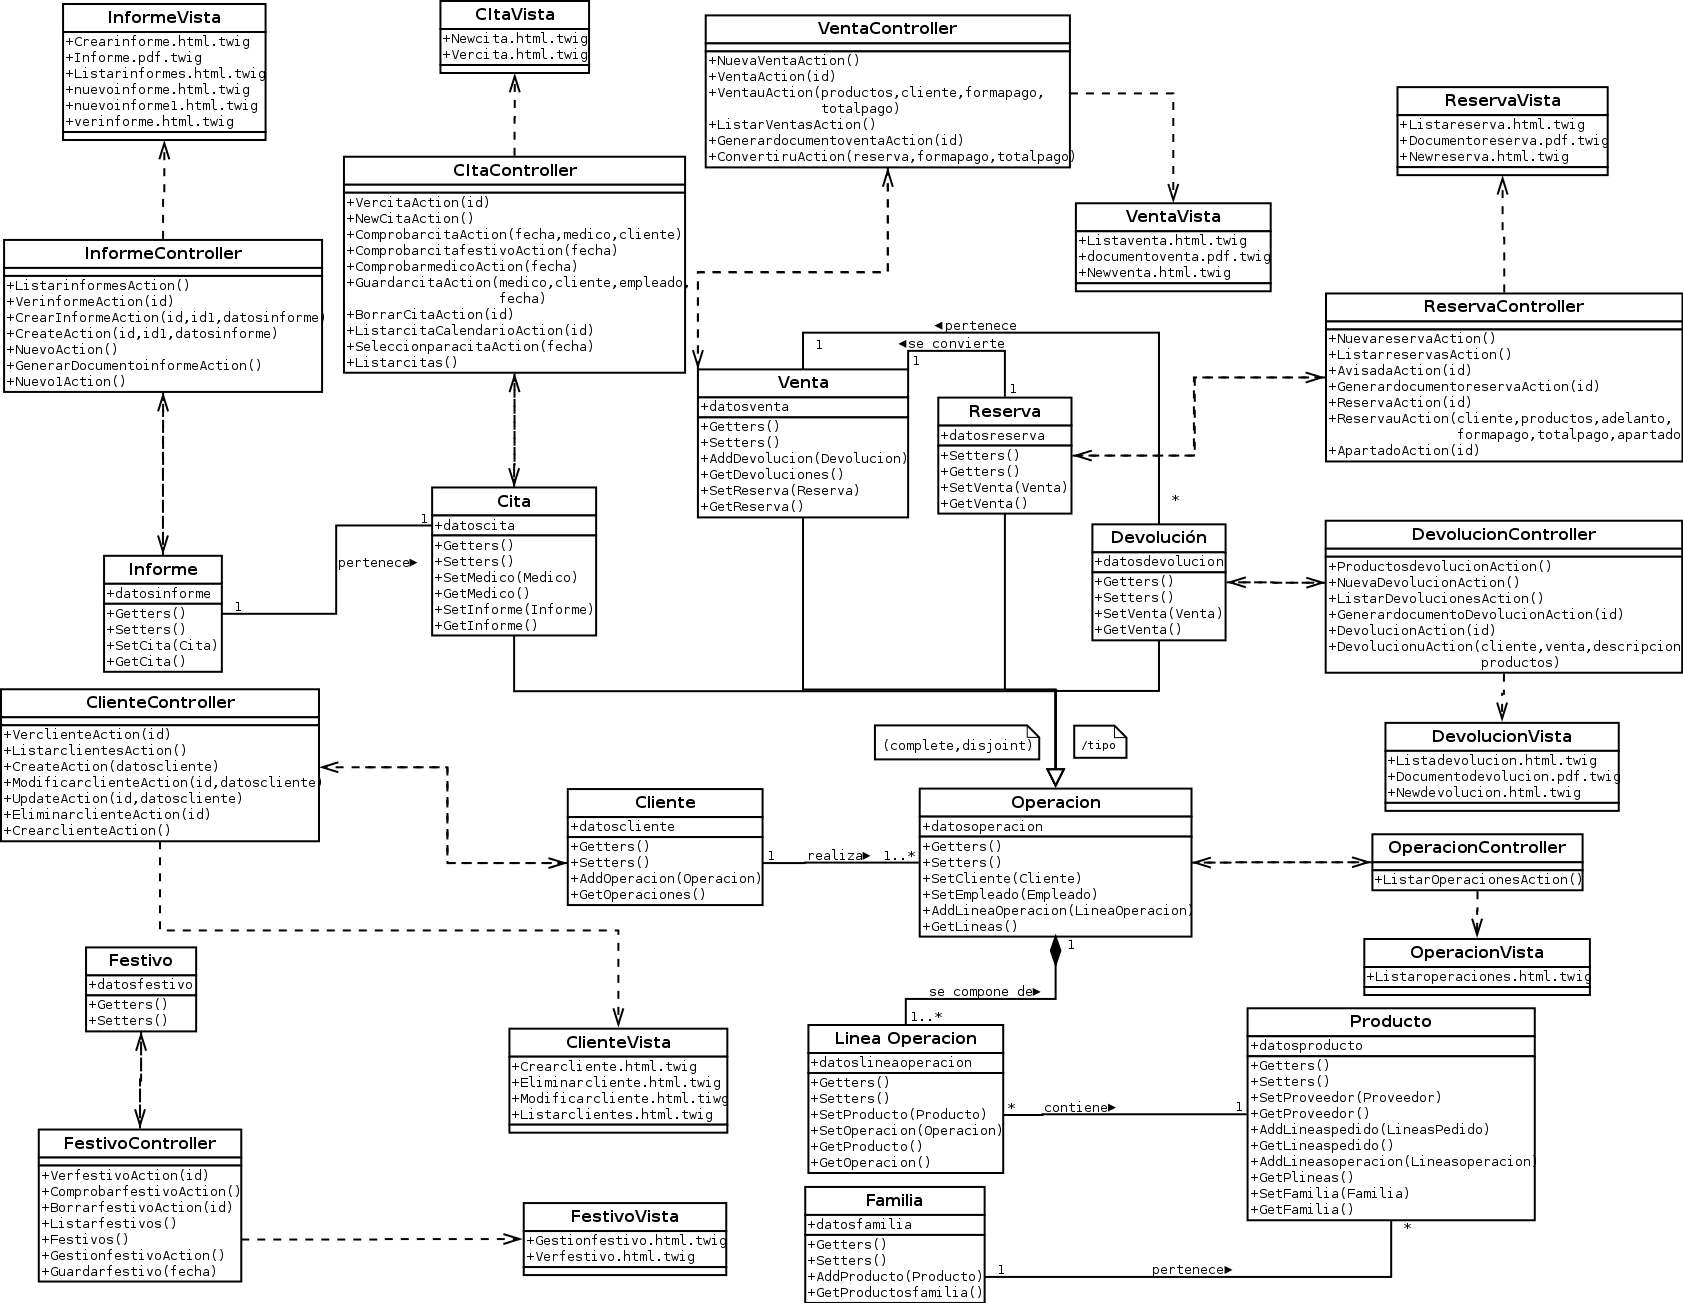
\includegraphics[angle=-90,scale=0.31]{diagramaclases1.png}
  \caption{Diagrama de clases de diseño 1}
  \label{a}
\end{figure}

\begin{figure}[!htb]
  \centering
    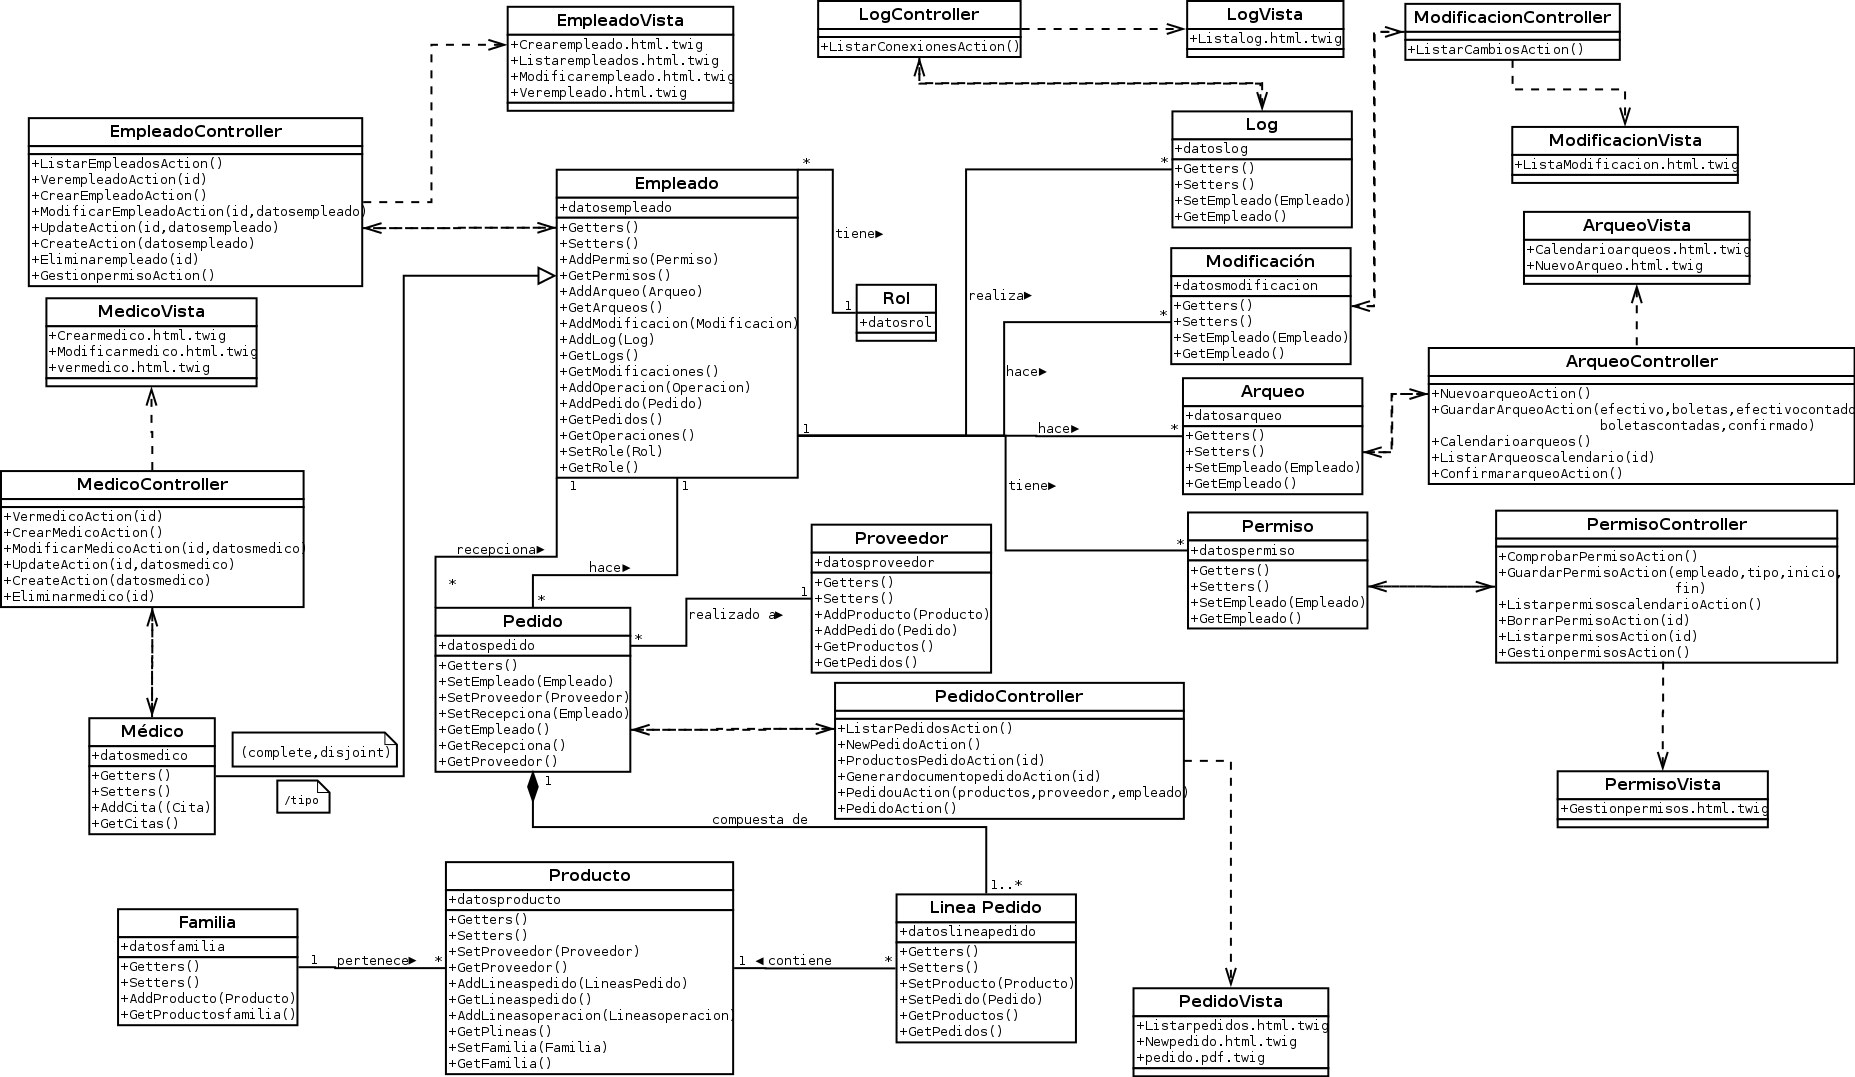
\includegraphics[angle=-90,scale=0.34]{diagramaclases2.png}
  \caption{Diagrama de clases de diseño 2}
  \label{a}
\end{figure}

\clearpage
\subsection{Diagramas de interacción}
A continuación se estudiarán los diagramas de interacción de sistemas de la aplicación de los casos de uso estudiados. Solo detallaremos algunos ya que muchos son similares, sobretodo los alternativos, y por lo tanto no aportan información. Omitiremos los diagramas de proveedores, familias y productos.\\
\begin{itemize}
\item \textbf{Caso de uso: Registrar cliente}
\begin{figure}[!htb]
  \centering
    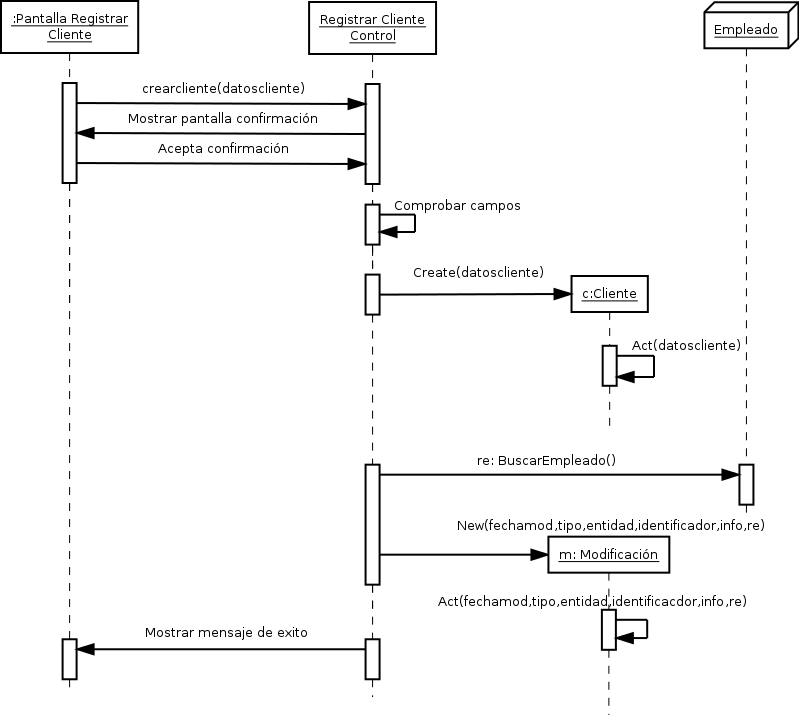
\includegraphics[scale=0.5]{registrarcliente.png}
  \caption{Diagrama de interacción. Caso de uso: Registrar cliente}
  \label{a}
\end{figure}
\clearpage
\item \textbf{Caso de uso: Registrar cliente - Alternativo 1}
\begin{figure}[!htb]
  \centering
    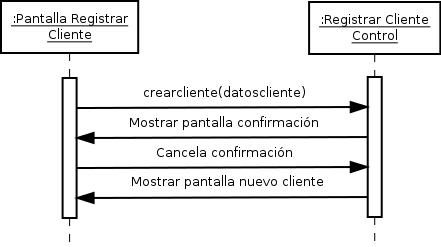
\includegraphics[scale=0.5]{registrarcliente1.png}
  \caption{Diagrama de interacción. Caso de uso: Registrar cliente - Alternativo 1}
  \label{a}
\end{figure}
\item \textbf{Caso de uso: Registrar cliente - Alternativo 2}
\begin{figure}[!htb]
  \centering
    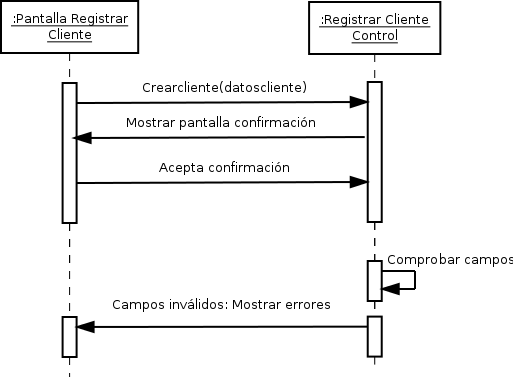
\includegraphics[scale=0.5]{registrarcliente2.png}
  \caption{Diagrama de interacción. Caso de uso: Registrar cliente - Alternativo 2}
  \label{a}
\end{figure}
\clearpage
\item \textbf{Caso de uso: Modificar cliente}
\begin{figure}[!htb]
  \centering
    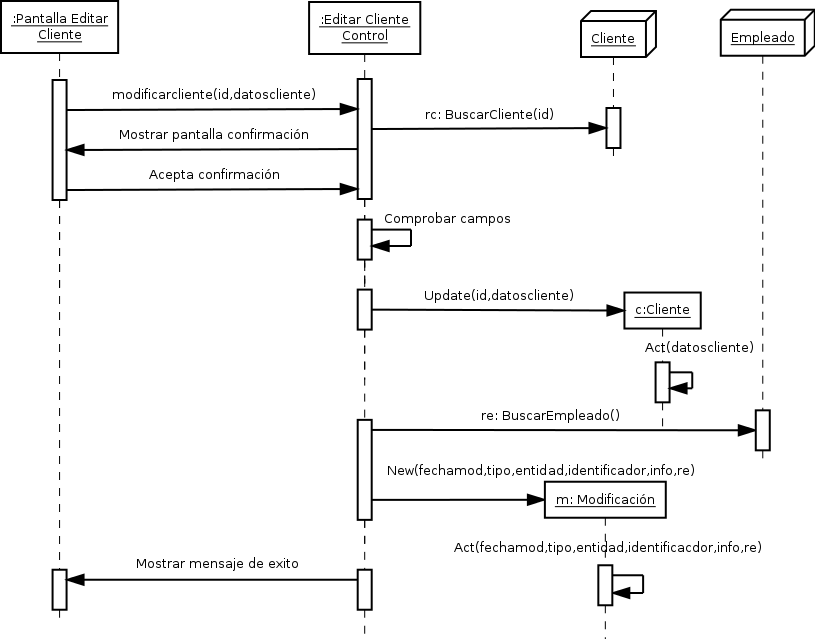
\includegraphics[scale=0.5]{editarcliente.png}
  \caption{Diagrama de interacción. Caso de uso: Modificar cliente}
  \label{a}
\end{figure}

\newpage
\item \textbf{Caso de uso: Modificar cliente - Alternativo 1}
\begin{figure}[!htb]
  \centering
    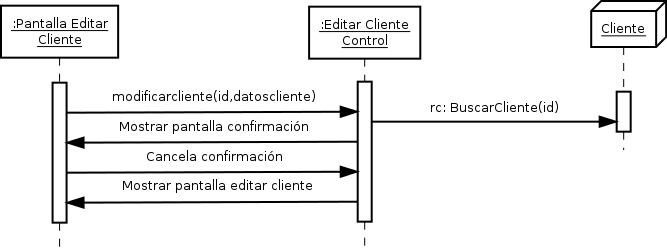
\includegraphics[scale=0.5]{editarcliente1.png}
  \caption{Diagrama de interacción. Caso de uso: Modificar cliente - Alternativo 1}
  \label{a}
\end{figure}

\item \textbf{Caso de uso: Modificar cliente - Alternativo 2}

\begin{figure}[!htb]
  \centering
    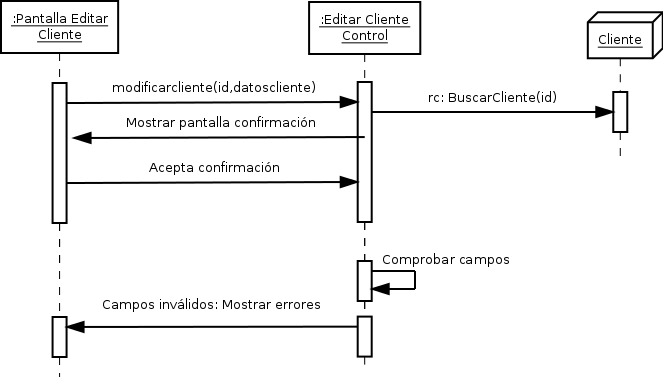
\includegraphics[scale=0.5]{editarcliente2.png}
  \caption{Diagrama de interacción. Caso de uso: Modificar cliente - Alternativo 2}
  \label{a}
\end{figure}

\newpage
\item \textbf{Caso de uso: Borrar cliente}
\begin{figure}[!htb]
  \centering
    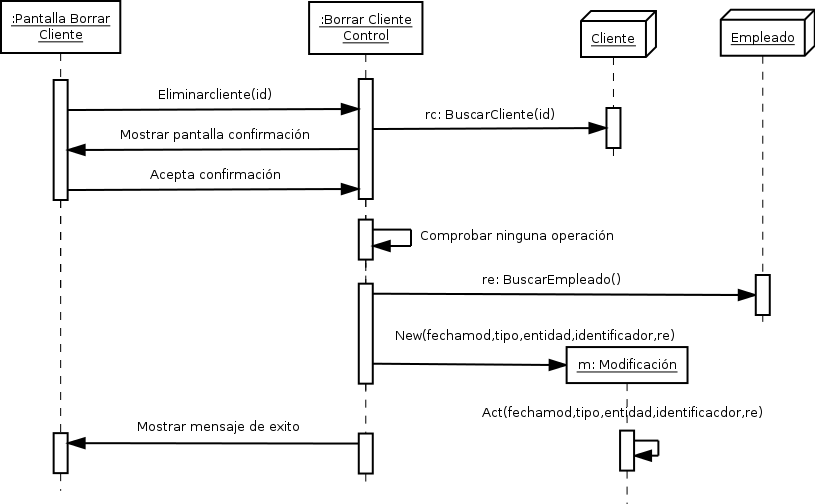
\includegraphics[scale=0.5]{borrarcliente.png}
  \caption{Diagrama de interacción. Caso de uso: Borrar cliente}
  \label{a}
\end{figure}

\item \textbf{Caso de uso: Borrar cliente - Alternativo 1}
\begin{figure}[!htb]
  \centering
    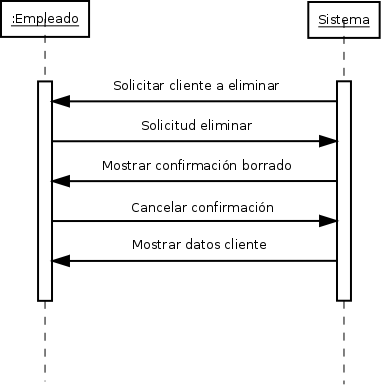
\includegraphics[scale=0.5]{borrarcliente1.png}
  \caption{Diagrama de interacción. Caso de uso: Borrar cliente - Alternativo 1}
  \label{a}
\end{figure}
\clearpage
\item \textbf{Caso de uso: Borrar cliente - Alternativo 2}
\begin{figure}[!htb]
  \centering
    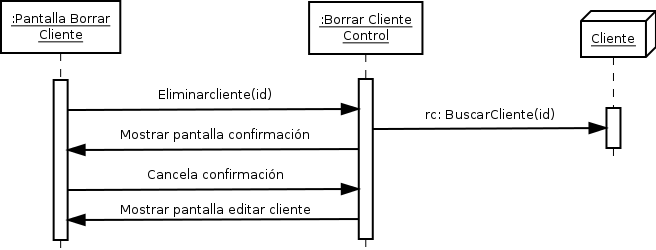
\includegraphics[scale=0.5]{borrarcliente2.png}
  \caption{Diagrama de interacción. Caso de uso: Borrar cliente - Alternativo 2}
  \label{a}
\end{figure}

\item \textbf{Caso de uso: Ver cliente}
\begin{figure}[!htb]
  \centering
    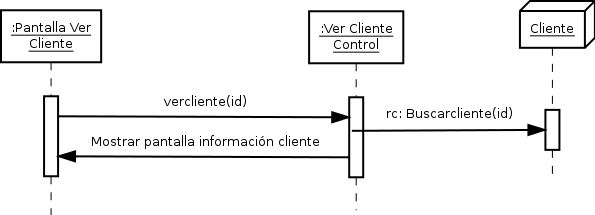
\includegraphics[scale=0.5]{vercliente.png}
  \caption{Diagrama de interacción. Caso de uso: Ver cliente}
  \label{a}
\end{figure}

\item \textbf{Caso de uso: Listar clientes}
\begin{figure}[!htb]
  \centering
    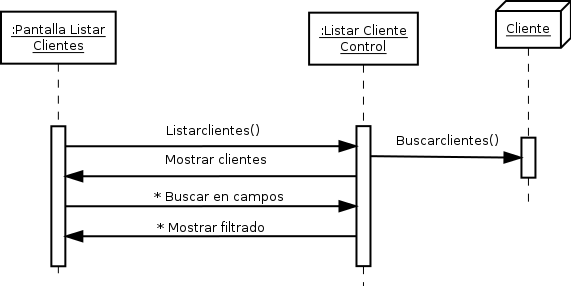
\includegraphics[scale=0.5]{listarcliente.png}
  \caption{Diagrama de interacción. Caso de uso: Listar clientes}
  \label{a}
\end{figure}
\newpage

\item \textbf{Caso de uso: Registrar Venta}
\begin{figure}[!htb]
  \centering
    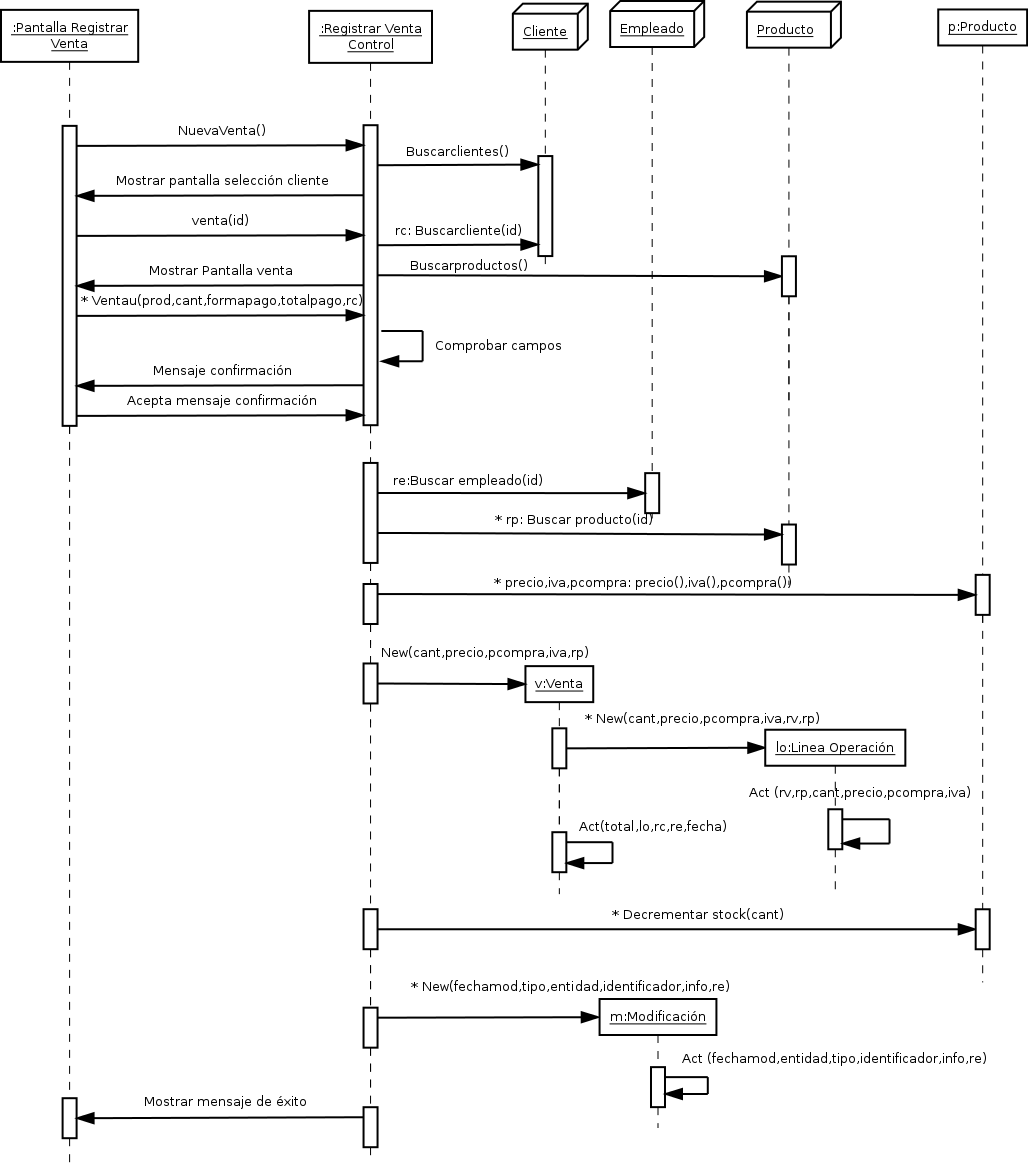
\includegraphics[scale=0.5]{registrarventa.png}
  \caption{Diagrama de interacción. Caso de uso: Registrar venta}
  \label{a}
\end{figure}
\newpage
\item \textbf{Caso de uso: Registrar Venta - Alternativo 1}
\begin{figure}[!htb]
  \centering
    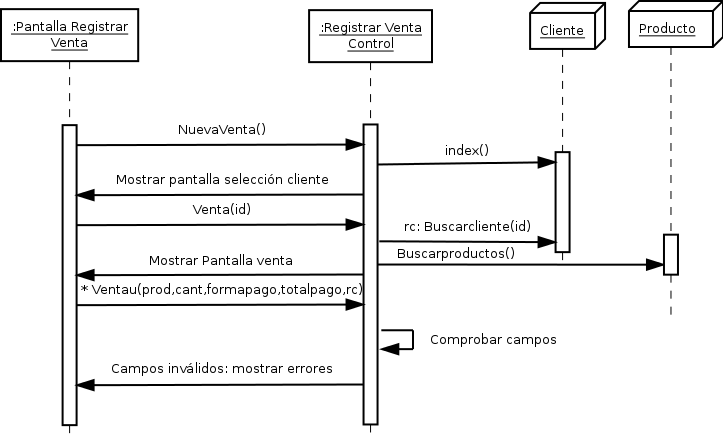
\includegraphics[scale=0.5]{registrarventa3.png}
  \caption{Diagrama de interacción. Caso de uso: Registrar venta - Alternativo 1}
  \label{a}
\end{figure}
\item \textbf{Caso de uso: Registrar Venta - Alternativo 2}
\begin{figure}[!htb]
  \centering
    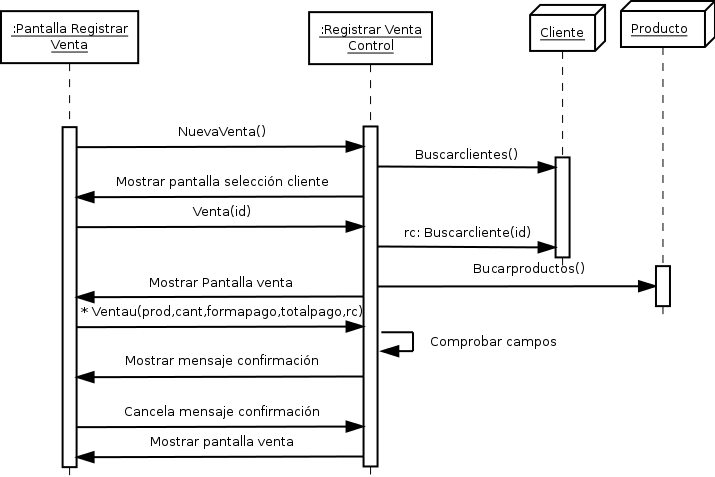
\includegraphics[scale=0.5]{registrarventa2.png}
  \caption{Diagrama de interacción. Caso de uso: Registrar venta - Alternativo 2}
  \label{a}
\end{figure}

\newpage
\item \textbf{Caso de uso: Registrar Venta - Alternativo 3}
\begin{figure}[!htb]
  \centering
    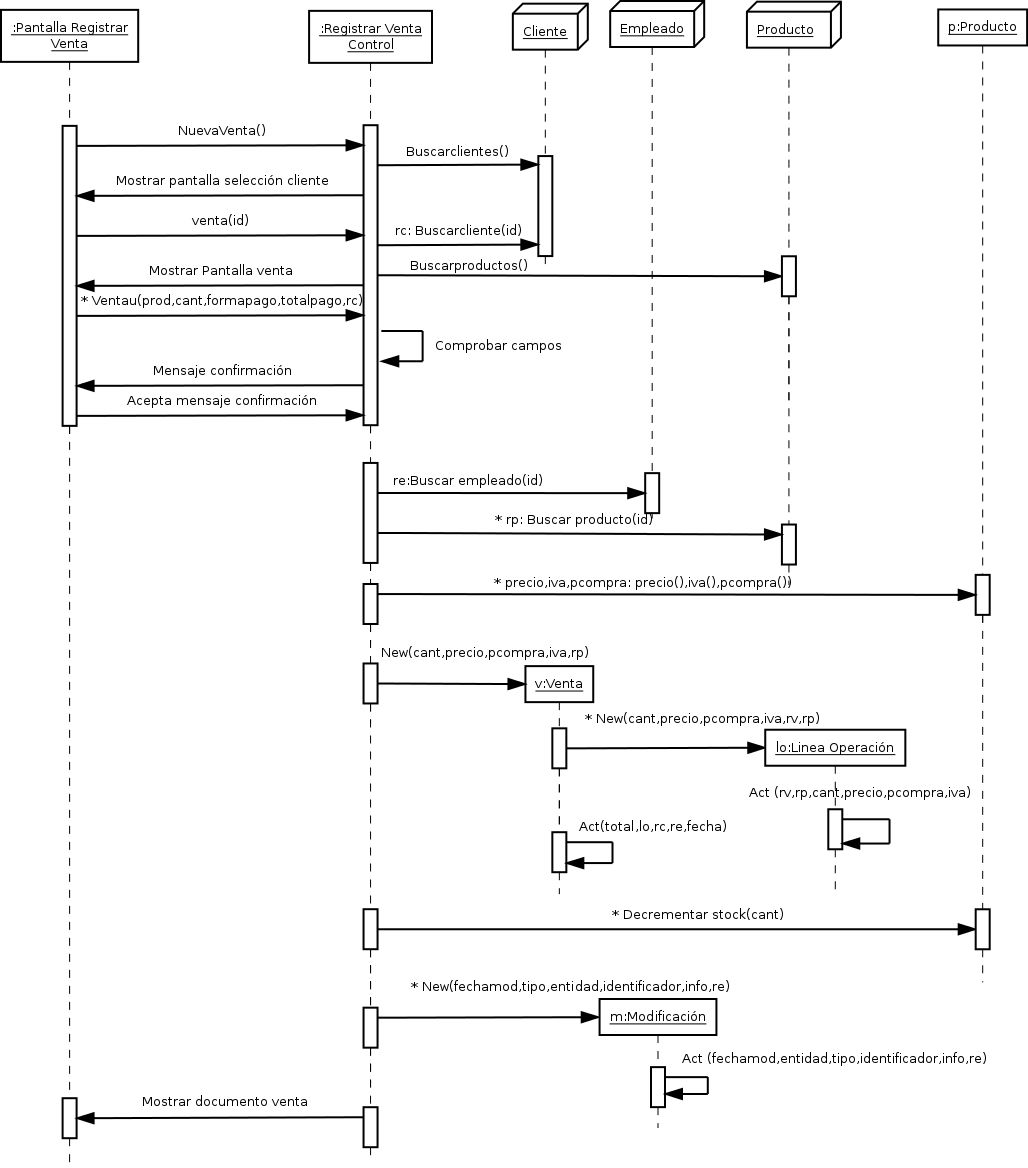
\includegraphics[scale=0.5]{registrarventa1.png}
  \caption{Diagrama de interacción. Caso de uso: Registrar venta - Alternativo 3}
  \label{a}
\end{figure}

\newpage
\item \textbf{Caso de uso: Listar Ventas}
\begin{figure}[!htb]
  \centering
    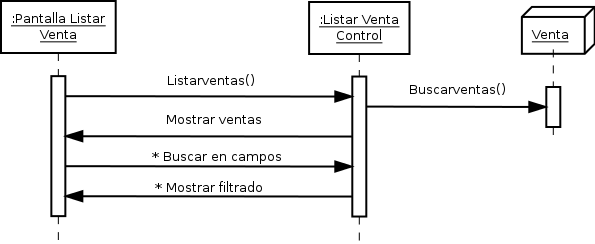
\includegraphics[scale=0.5]{listarventa.png}
  \caption{Diagrama de interacción. Caso de uso: Listar ventas}
  \label{a}
\end{figure}

\item \textbf{Caso de uso: Generar documento venta}
\begin{figure}[!htb]
  \centering
    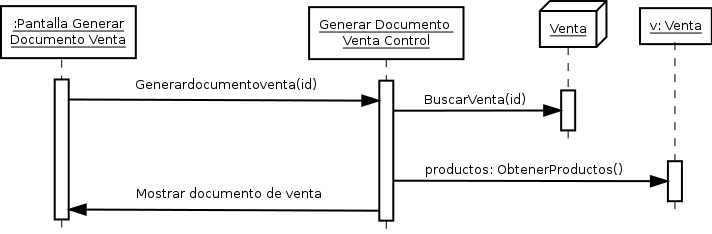
\includegraphics[scale=0.5]{generarfactura.png}
  \caption{Diagrama de interacción. Caso de uso: Generar documento venta}
  \label{a}
\end{figure}

\newpage
\item \textbf{Caso de uso: Registrar Devolución}
\begin{figure}[!htb]
  \centering
    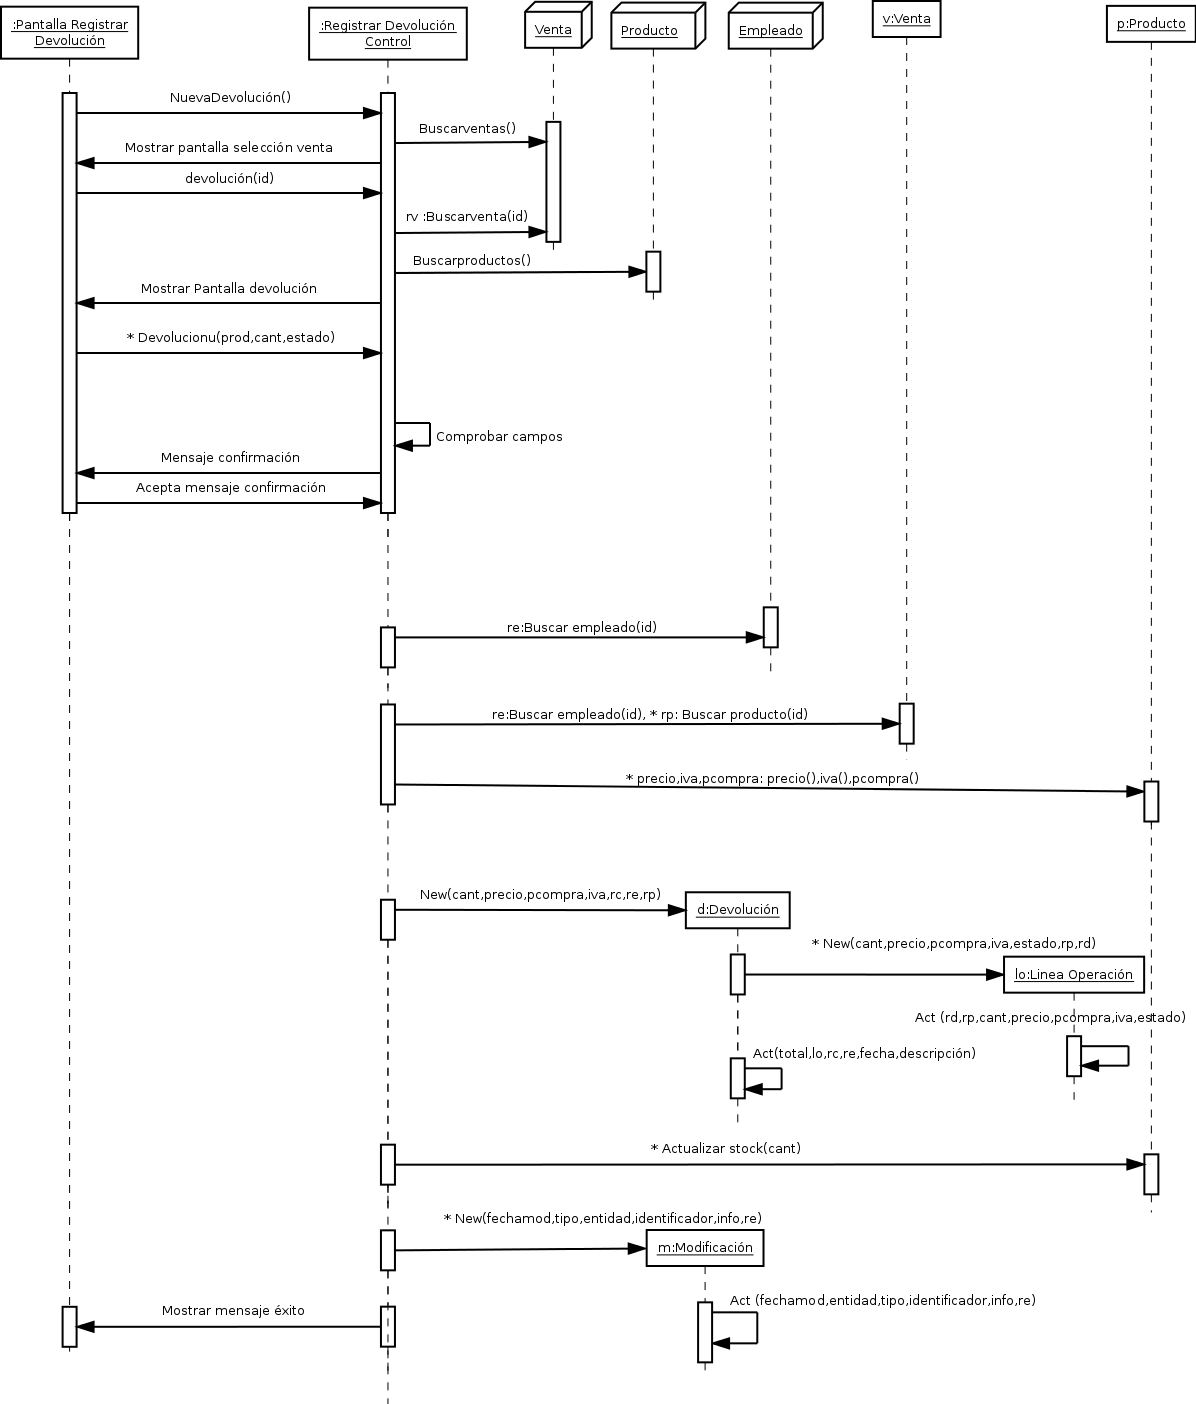
\includegraphics[scale=0.4]{registrardevolucion.png}
  \caption{Diagrama de interacción. Caso de uso: Registrar devolución}
  \label{a}
\end{figure}

\newpage
\item \textbf{Caso de uso: Registrar Devolución Alternativo 1}
\begin{figure}[!htb]
  \centering
    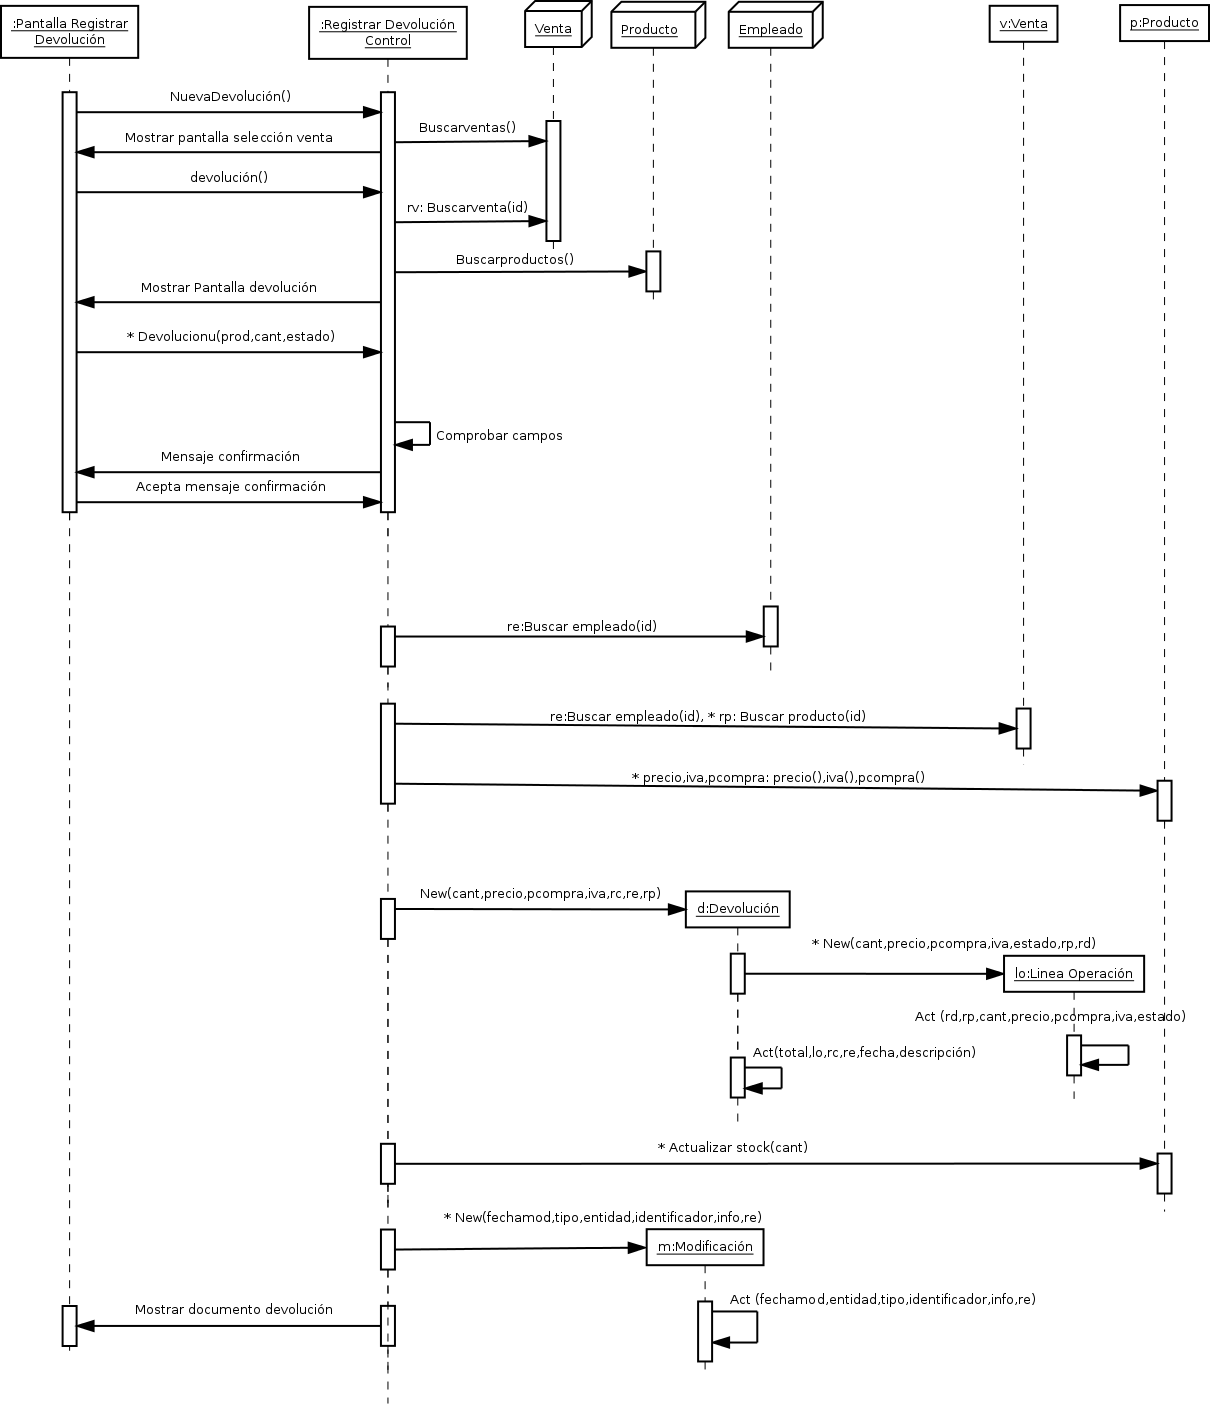
\includegraphics[scale=0.4]{registrardevolucion1.png}
  \caption{Diagrama de interacción. Caso de uso: Registrar devolución - Alternativo 1}
  \label{a}
\end{figure}
\clearpage
\item \textbf{Caso de uso: Registrar Devolución - Alternativo 2}
\begin{figure}[!htb]
  \centering
    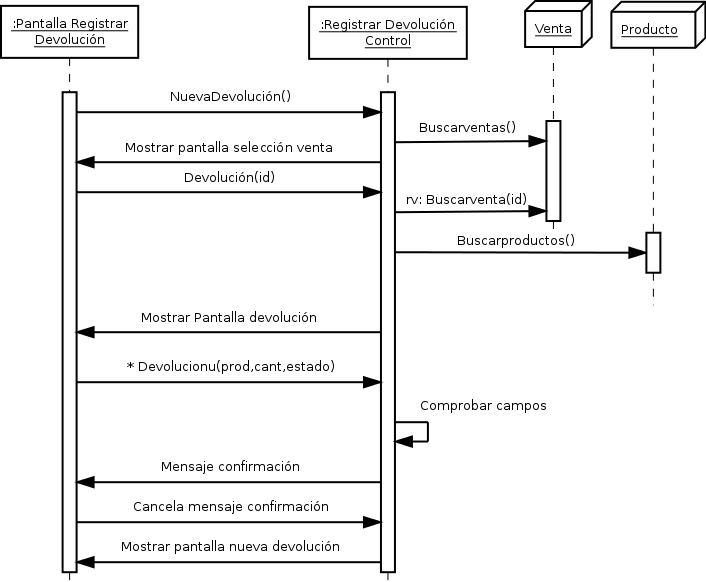
\includegraphics[scale=0.4]{registrardevolucion2.png}
  \caption{Diagrama de interacción. Caso de uso: Registrar devolución - Alternativo 2}
  \label{a}
\end{figure}

\item \textbf{Caso de uso: Registrar Devolución - Alternativo 3}
\begin{figure}[!htb]
  \centering
    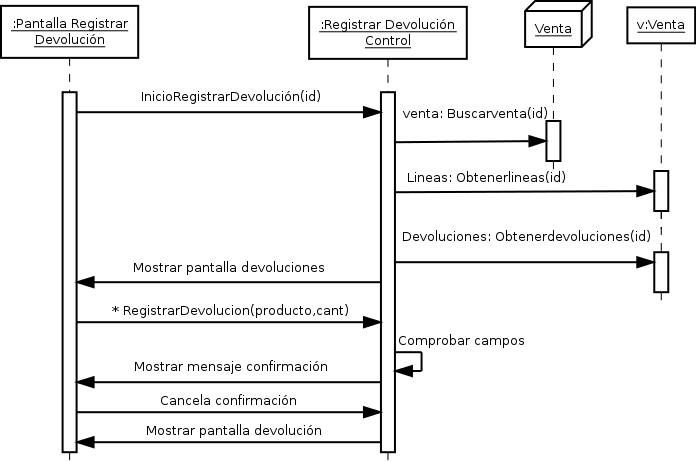
\includegraphics[scale=0.4]{registrardevolucion3.png}
  \caption{Diagrama de interacción. Caso de uso: Registrar devolución - Alternativo 3}
  \label{a}
\end{figure}

\newpage
\item \textbf{Caso de uso: Listar devoluciones}
\begin{figure}[!htb]
  \centering
    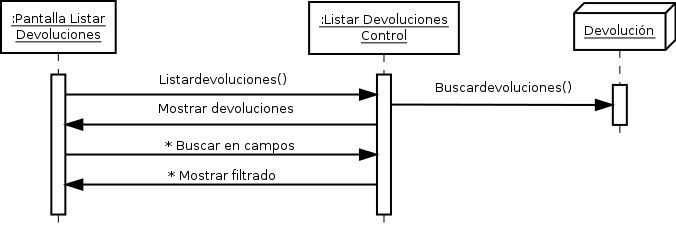
\includegraphics[scale=0.5]{listardevolucion.png}
  \caption{Diagrama de interacción. Caso de uso: Listar devoluciones}
  \label{a}
\end{figure}

\item \textbf{Caso de uso: Generar documento devolución}
\begin{figure}[!htb]
  \centering
    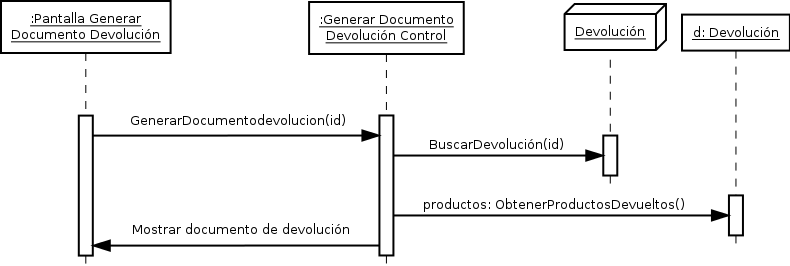
\includegraphics[scale=0.5]{generardocumento.png}
  \caption{Diagrama de interacción. Caso de uso: Generar documento devolución}
  \label{a}
\end{figure}

\item \textbf{Caso de uso: Ver productos devueltos}
\begin{figure}[!htb]
  \centering
    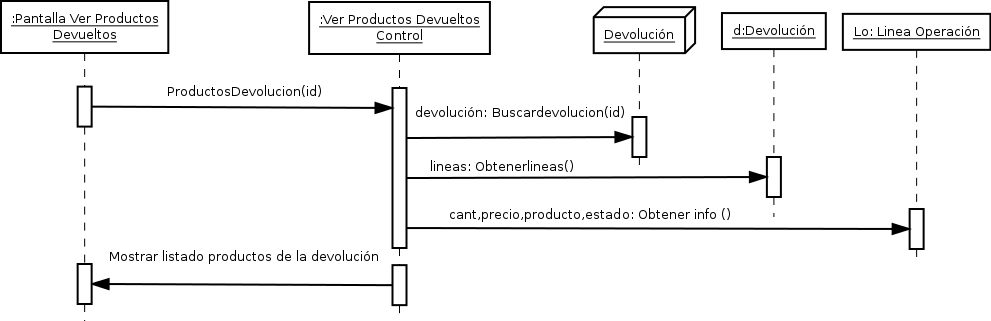
\includegraphics[scale=0.5]{verproductosdevueltos.png}
  \caption{Diagrama de interacción. Caso de uso: Ver productos devueltos}
  \label{a}
\end{figure}
\newpage
\item \textbf{Caso de uso: Registrar Reserva}
\begin{figure}[!htb]
  \centering
    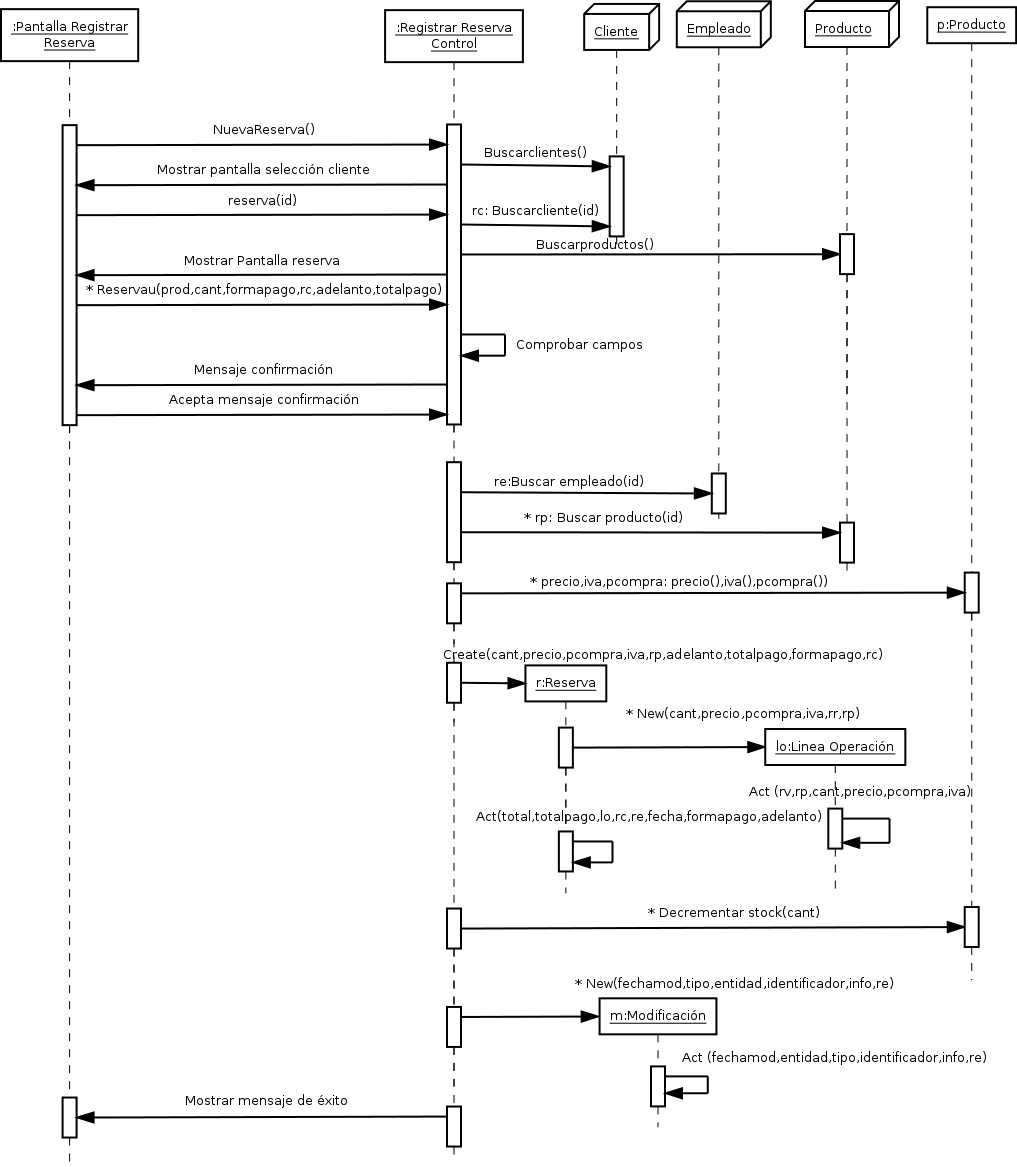
\includegraphics[scale=0.5]{registrarreserva.png}
  \caption{Diagrama de interacción. Caso de uso: Registrar reserva}
  \label{a}
\end{figure}
\newpage
\item \textbf{Caso de uso: Registrar Reserva - Alternativo 1}
\begin{figure}[!htb]
  \centering
    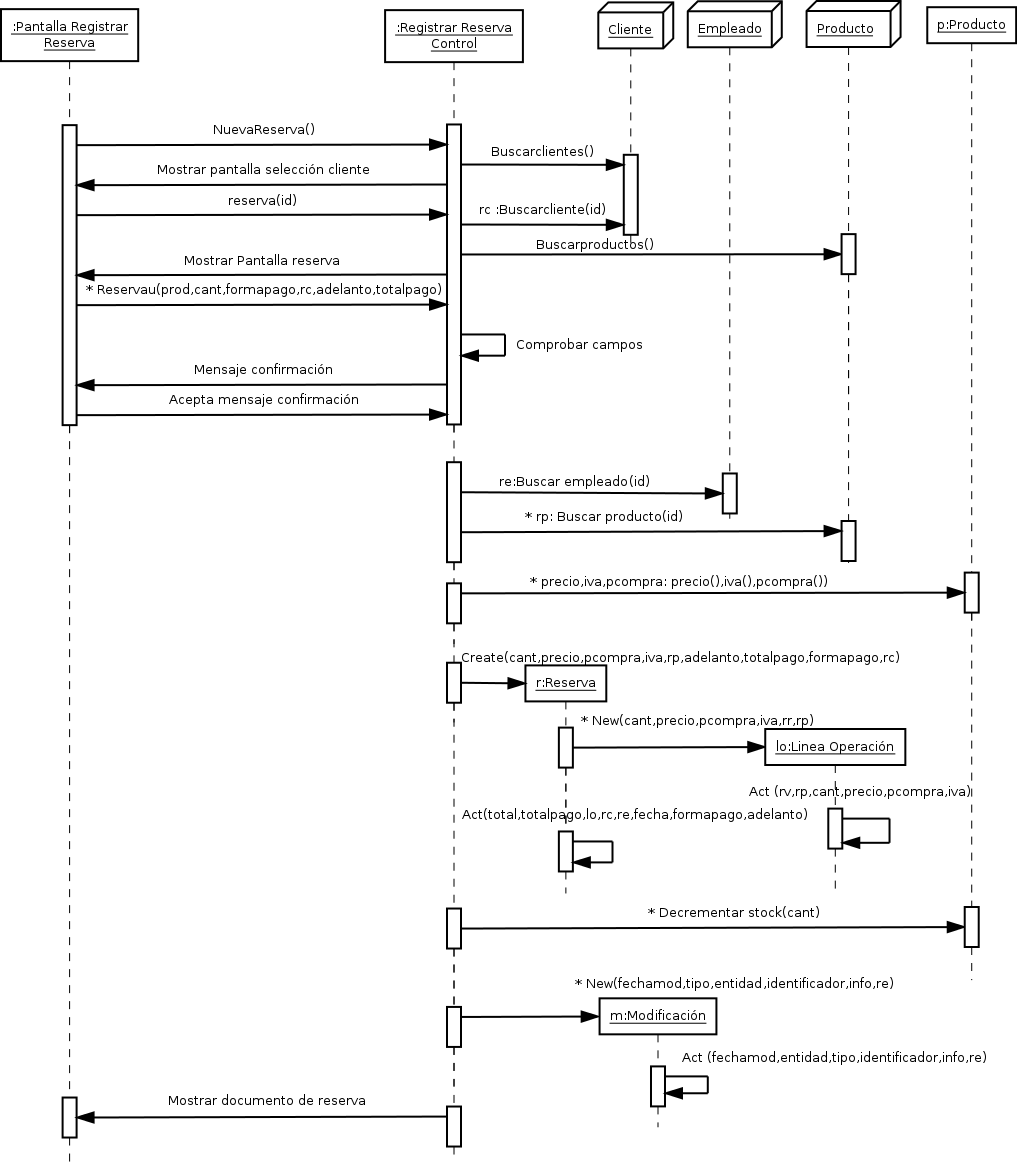
\includegraphics[scale=0.5]{registrarreserva3.png}
  \caption{Diagrama de interacción. Caso de uso: Registrar reserva - Alternativo 1}
  \label{a}
\end{figure}
\item \textbf{Caso de uso: Registrar Reserva - Alternativo 2}
\begin{figure}[!htb]
  \centering
    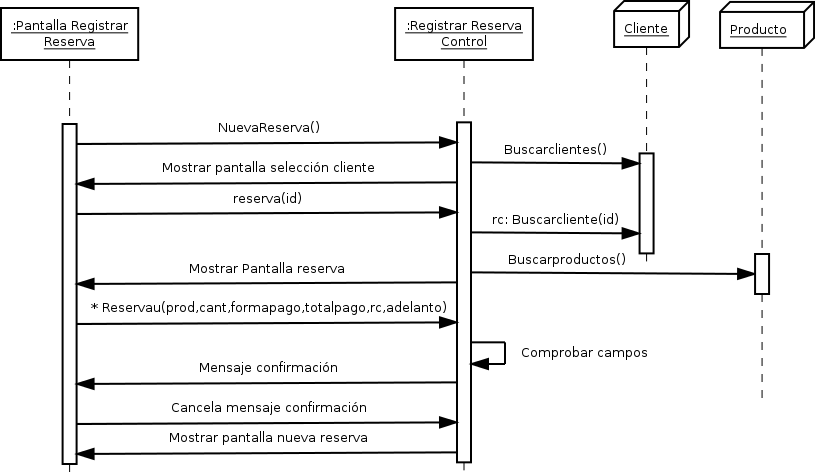
\includegraphics[scale=0.5]{registrarreserva2.png}
  \caption{Diagrama de interacción. Caso de uso: Registrar reserva - Alternativo 2}
  \label{a}
\end{figure}

\item \textbf{Caso de uso: Registrar Reserva - Alternativo 3}
\begin{figure}[!htb]
  \centering
    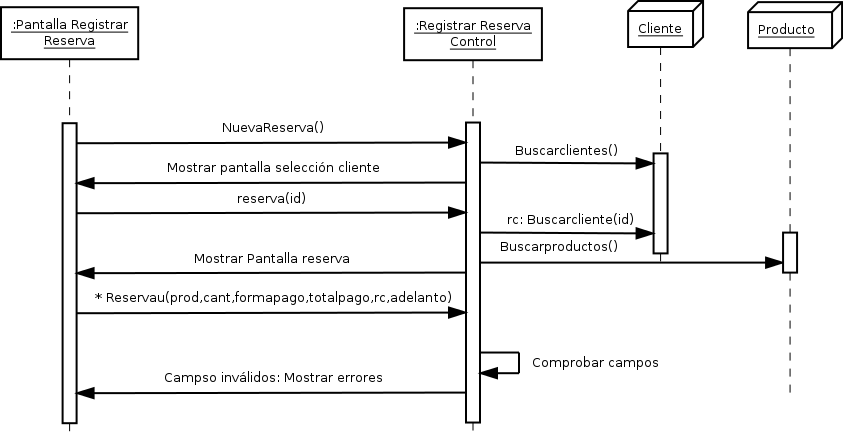
\includegraphics[scale=0.5]{registrarreserva1.png}
  \caption{Diagrama de interacción. Caso de uso: Registrar reserva -Alternativo 3}
  \label{a}
\end{figure}

\newpage
\item \textbf{Caso de uso: Listar reservas}
\begin{figure}[!htb]
  \centering
    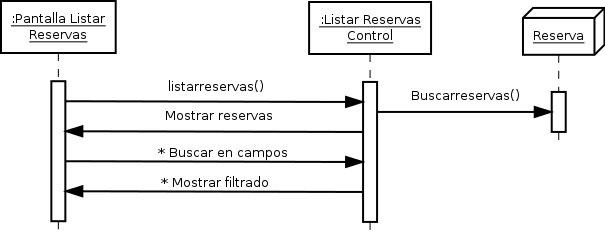
\includegraphics[scale=0.5]{listarreserva.png}
  \caption{Diagrama de interacción. Caso de uso: Listar reservas}
  \label{a}
\end{figure}

\item \textbf{Caso de uso: Generar documento reserva}
\begin{figure}[!htb]
  \centering
    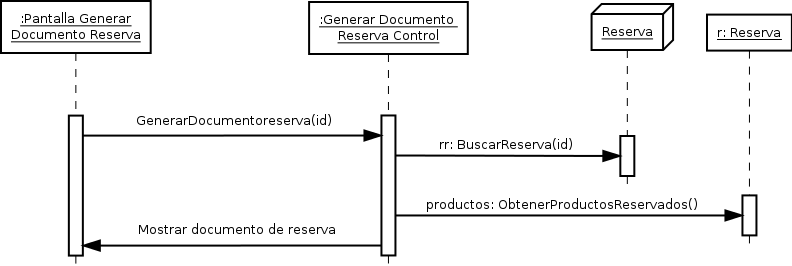
\includegraphics[scale=0.5]{generardocumentoreserva.png}
  \caption{Diagrama de interacción. Caso de uso: Generar documento reserva}
  \label{a}
\end{figure}

\item \textbf{Caso de uso: Ver productos reserva}
\begin{figure}[!htb]
  \centering
    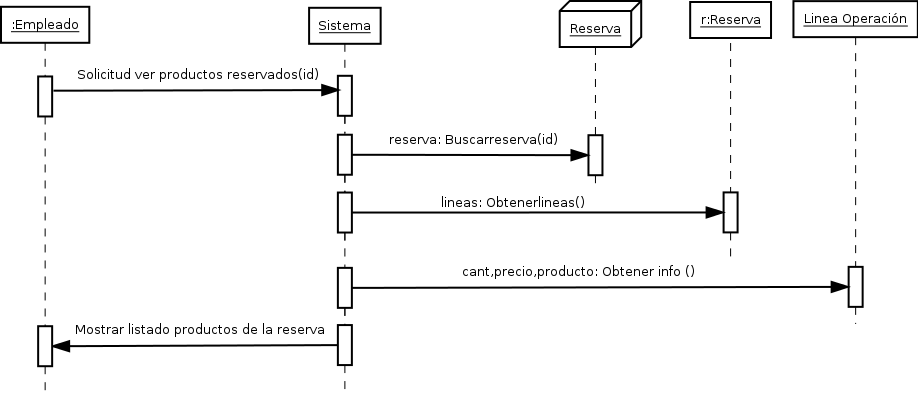
\includegraphics[scale=0.5]{verproductosreserva.png}
  \caption{Diagrama de interacción. Caso de uso:  Ver productos reserva}
  \label{a}
\end{figure}

\newpage

\item \textbf{Caso de uso: Registrar cita}
\begin{figure}[!htb]
  \centering
    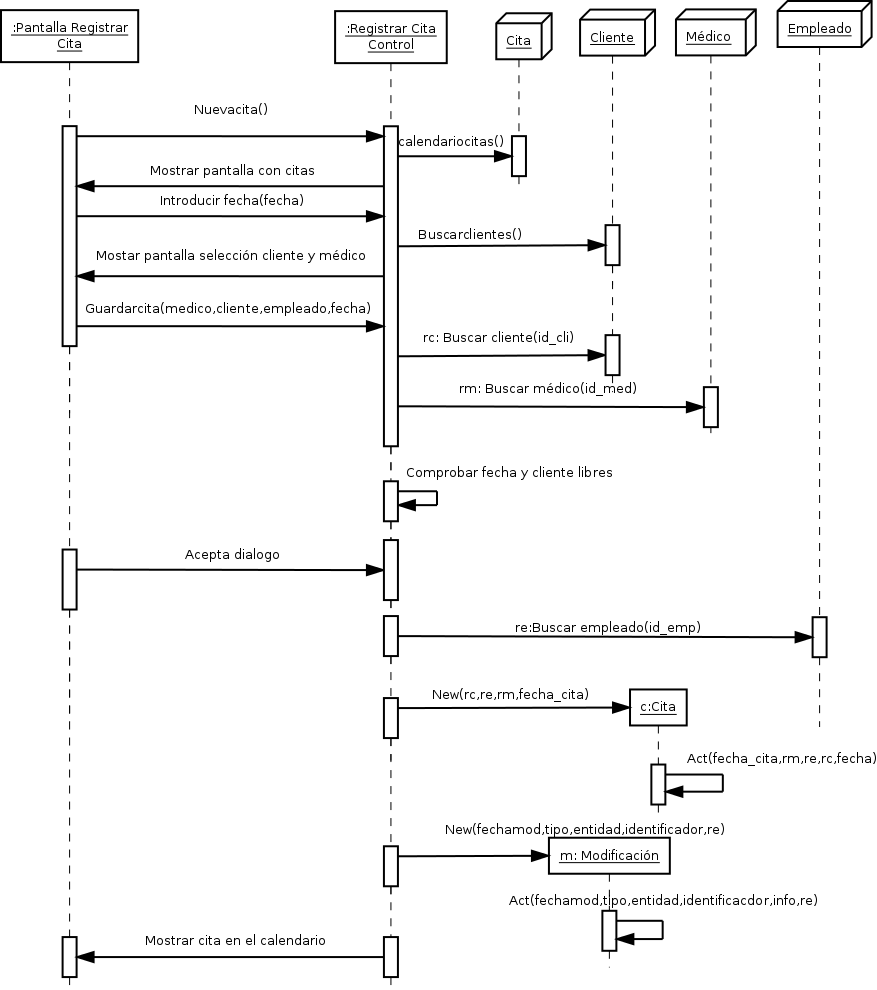
\includegraphics[scale=0.45]{registrarcita.png}
  \caption{Diagrama de interacción. Caso de uso: Registrar cita}
  \label{a}
\end{figure}

\newpage
\item \textbf{Caso de uso: Registrar cita - Alternativo 1}
\begin{figure}[!htb]
  \centering
    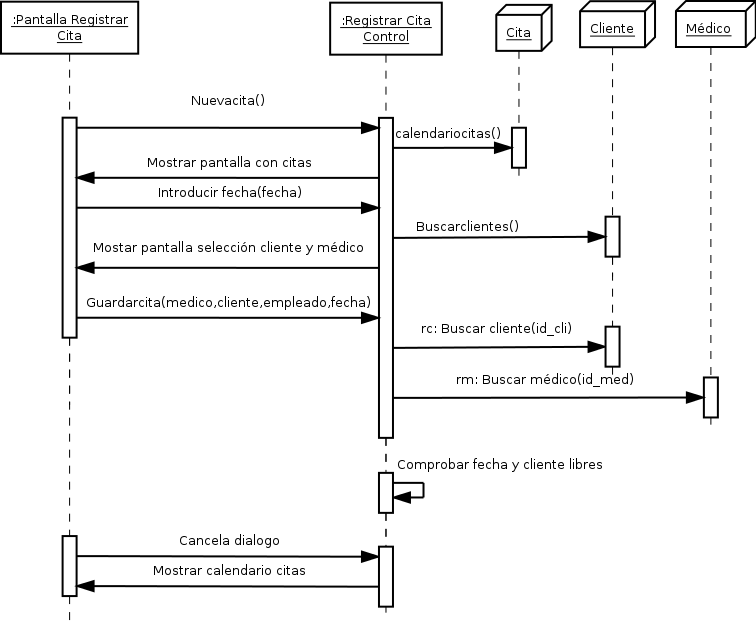
\includegraphics[scale=0.5]{registrarcita1.png}
  \caption{Diagrama de interacción. Caso de uso: Registrar cita - Alternativo 1}
  \label{a}
\end{figure}

\newpage
\item \textbf{Caso de uso: Registrar cita - Alternativo 2}
\begin{figure}[!htb]
  \centering
    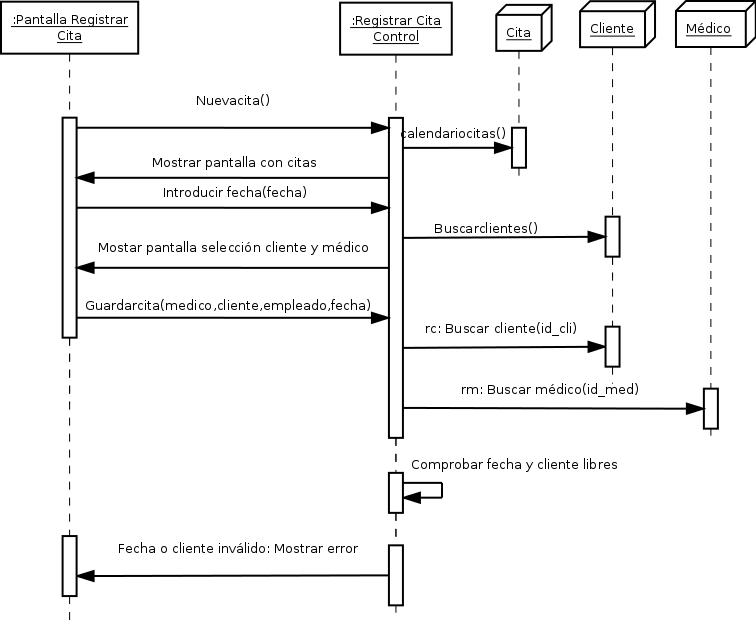
\includegraphics[scale=0.5]{registrarcita2.png}
  \caption{Diagrama de interacción. Caso de uso: Registrar cita - Alternativo 2}
  \label{a}
\end{figure}


\newpage
\item \textbf{Caso de uso: Ver Cita}
\begin{figure}[!htb]
  \centering
    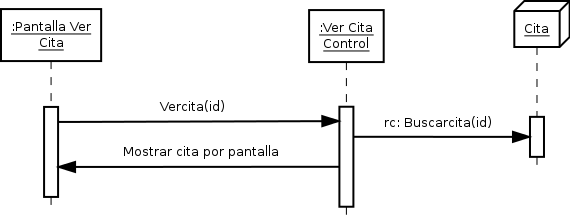
\includegraphics[scale=0.5]{vercita.png}
  \caption{Diagrama de interacción. Caso de uso: Ver cita}
  \label{a}
\end{figure}

\item \textbf{Caso de uso: Listar citas}
\begin{figure}[!htb]
  \centering
  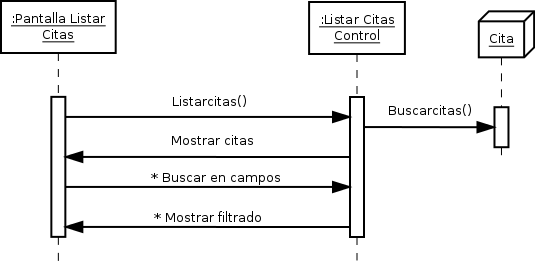
\includegraphics[scale=0.5]{listarcita.png}
  \caption{Diagrama de interacción. Caso de uso: Listar citas}
  \label{a}
\end{figure}

\item \textbf{Caso de uso: Listar informes}
\begin{figure}[!htb]
  \centering
  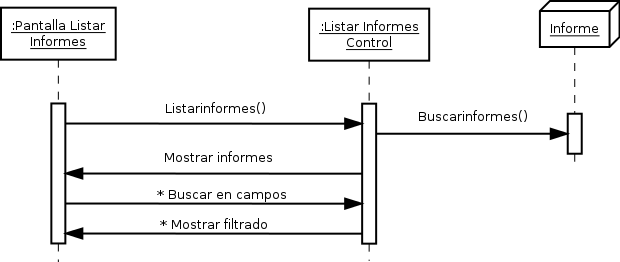
\includegraphics[scale=0.5]{listarinforme.png}
  \caption{Diagrama de interacción. Caso de uso: Listar informes}
  \label{a}
\end{figure}

\newpage
\item \textbf{Caso de uso: Generar informe con cita}
\begin{figure}[!htb]
  \centering
  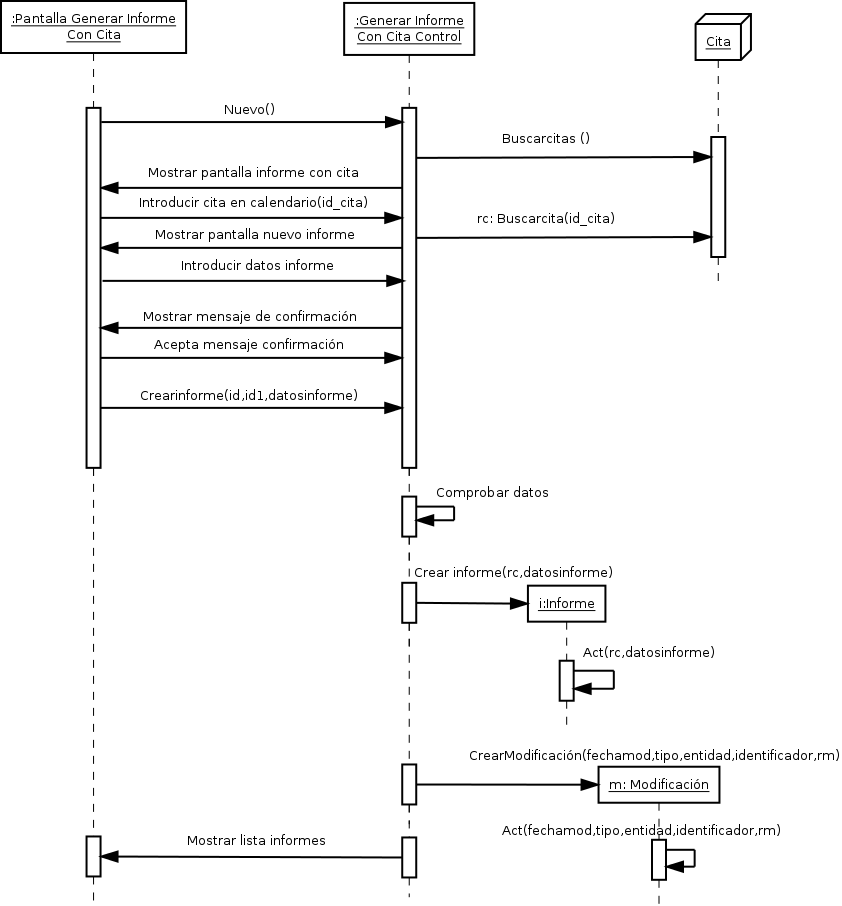
\includegraphics[scale=0.5]{registrarinformeconcita.png}
  \caption{Diagrama de interacción. Caso de uso: Generar informe con cita}
  \label{a}
\end{figure}
\newpage
\item \textbf{Caso de uso: Generar informe sin cita}
\begin{figure}[!htb]
  \centering
  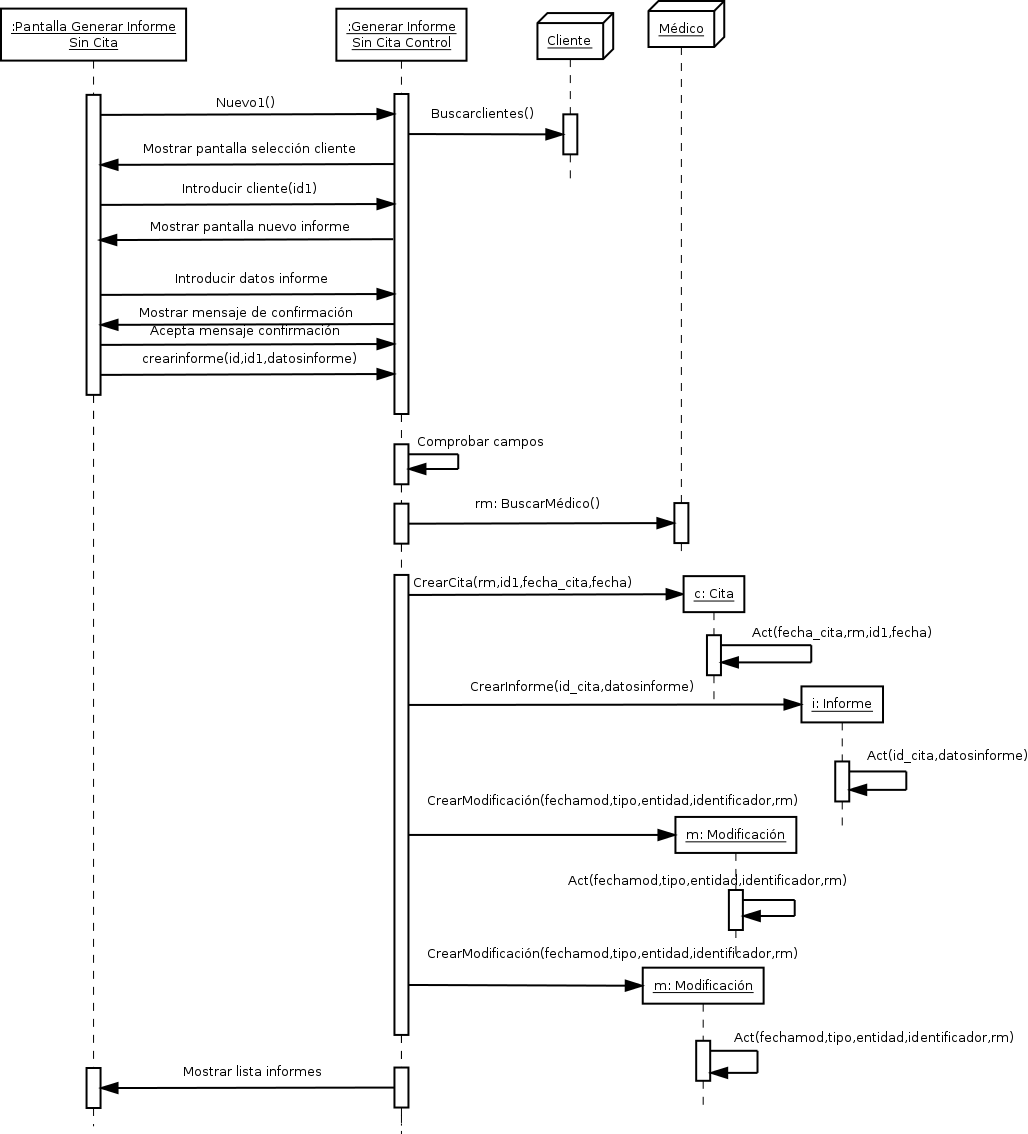
\includegraphics[scale=0.5]{registrarinformesincita.png}
  \caption{Diagrama de interacción. Caso de uso: Generar informe sin cita}
  \label{a}
\end{figure}

\newpage
\item \textbf{Caso de uso: Registrar Pedido}
\begin{figure}[!htb]
  \centering
    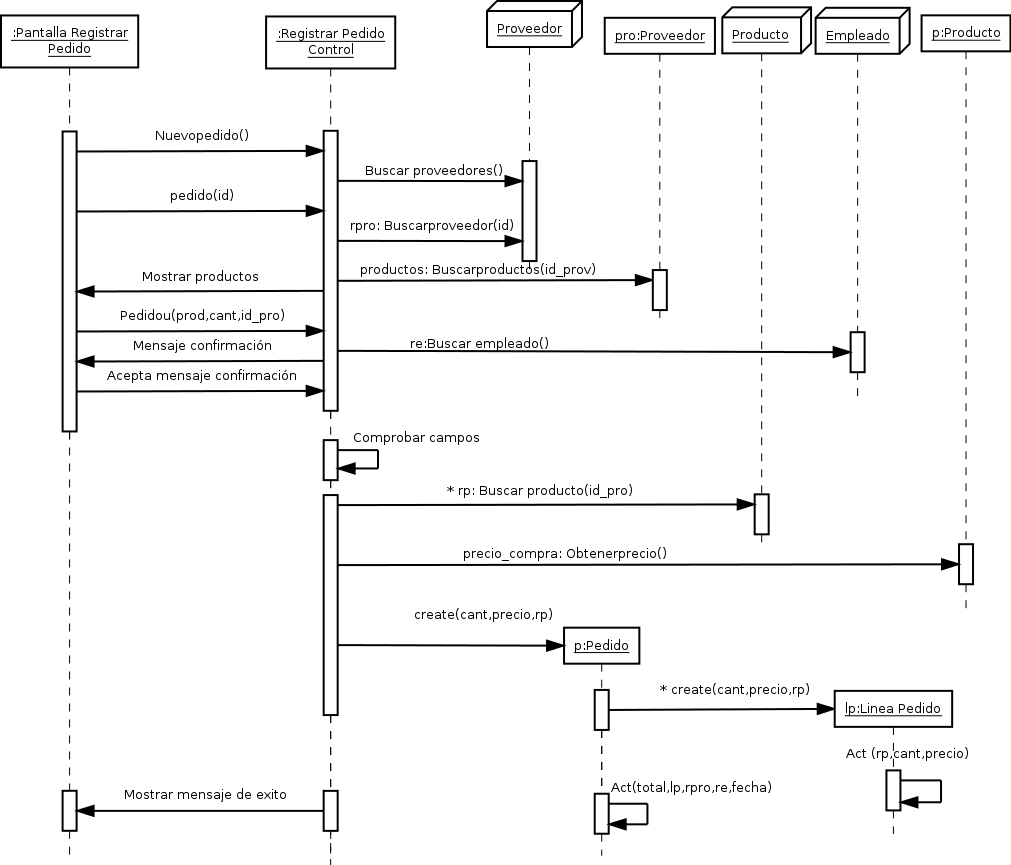
\includegraphics[scale=0.5]{registrarpedido.png}
  \caption{Diagrama de interacción. Caso de uso: Registrar pedido}
  \label{a}
\end{figure}
\newpage

\newpage
\item \textbf{Caso de uso: Registrar Pedido - Alternativo 1}
\begin{figure}[!htb]
  \centering
    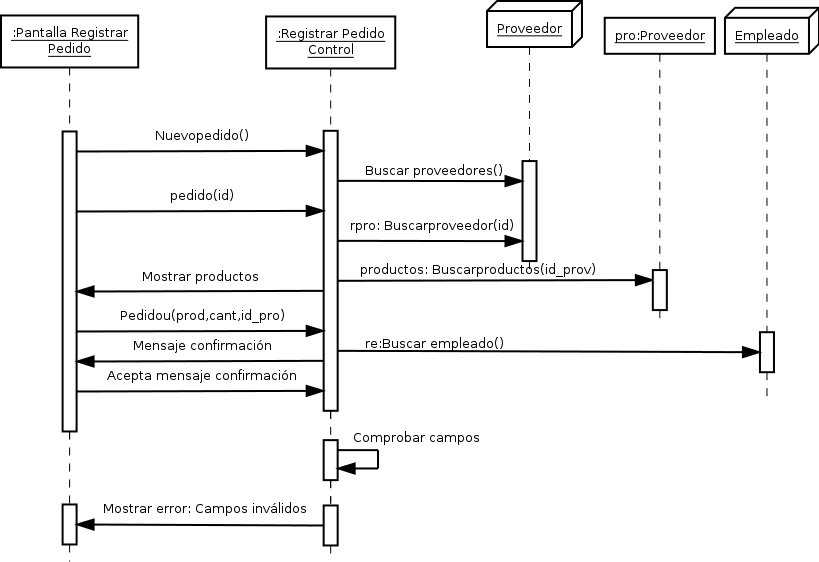
\includegraphics[scale=0.5]{registrarpedido2.png}
  \caption{Diagrama de interacción. Caso de uso: Registrar Pedido - Alternativo 1}
  \label{a}
\end{figure}

\item \textbf{Caso de uso: Registrar Pedido - Alternativo 2}
\begin{figure}[!htb]
  \centering
    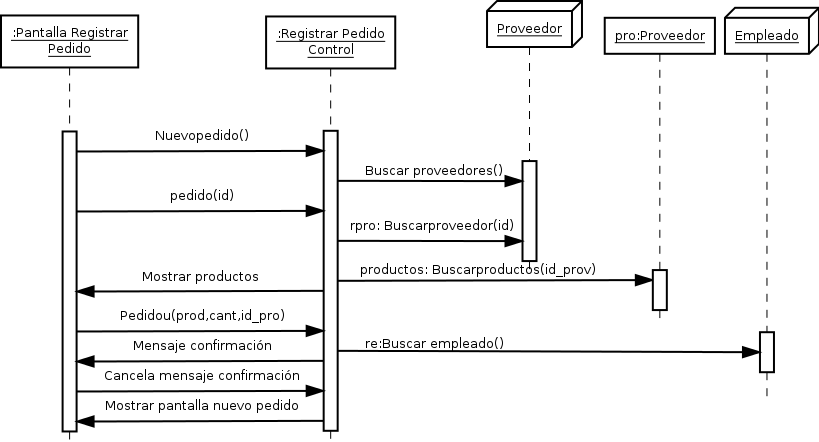
\includegraphics[scale=0.5]{registrarpedido3.png}
  \caption{Diagrama de interacción. Caso de uso: Registrar Pedido - Alternativo 2}
  \label{a}
\end{figure}

\newpage
\item \textbf{Caso de uso: Listar Pedidos}
\begin{figure}[!htb]
  \centering
    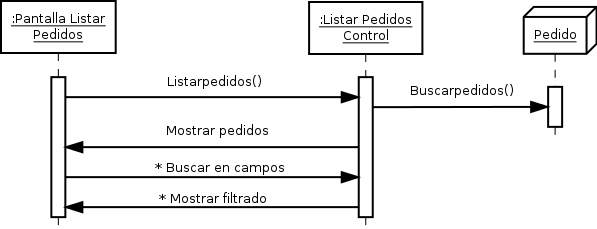
\includegraphics[scale=0.5]{listarpedido.png}
  \caption{Diagrama de interacción. Caso de uso: Listar pedidos}
  \label{a}
\end{figure}

\item \textbf{Caso de uso: Entrada al sistema}
\begin{figure}[!htb]
  \centering
    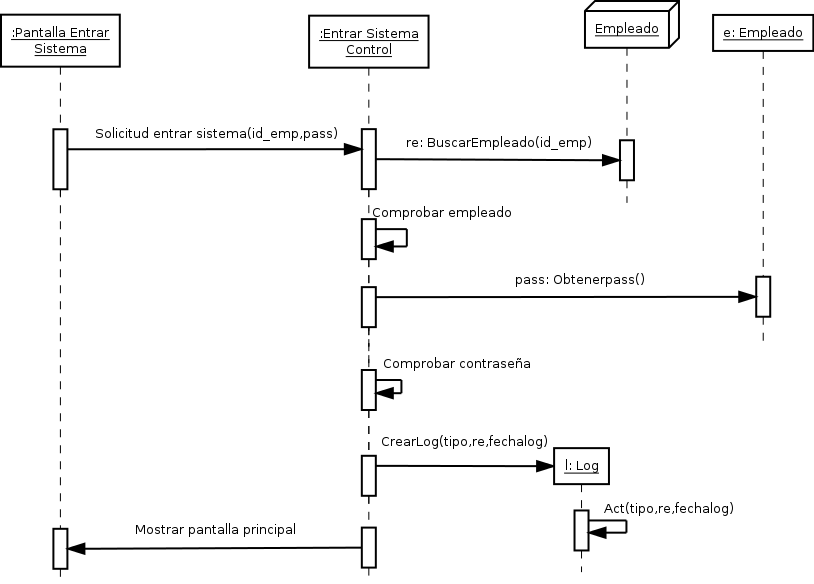
\includegraphics[scale=0.5]{entrarsistema.png}
  \caption{Diagrama de interacción. Caso de uso: Entrada al sistema}
  \label{a}
\end{figure}

\newpage
\item \textbf{Caso de uso: Entrada al sistema - Alternativo 1}
\begin{figure}[!htb]
  \centering
    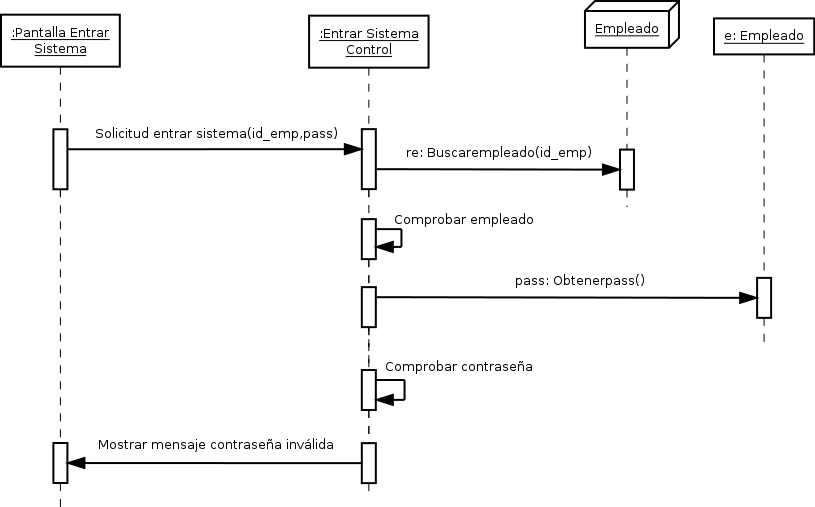
\includegraphics[scale=0.5]{entrarsistema1.png}
  \caption{Diagrama de interacción. Caso de uso: Entrada al sistema - Alternativo 1}
  \label{a}
\end{figure}

\item \textbf{Caso de uso: Entrada al sistema - Alternativo 2}
\begin{figure}[!htb]
  \centering
    \includegraphics[scale=0.5]{entrarsistema2.png}
  \caption{Diagrama de interacción. Caso de uso: Entrada al sistema - Alternativo 2}
  \label{a}
\end{figure}

\newpage
\item \textbf{Caso de uso: Salida del sistema}
\begin{figure}[!htb]
  \centering
    \includegraphics[scale=0.5]{salidasistema.png}
  \caption{Diagrama de interacción. Caso de uso: Salida del sistema}
  \label{a}
\end{figure}

\item \textbf{Caso de uso: Olvido contraseña}
\begin{figure}[!htb]
  \centering
    \includegraphics[scale=0.5]{olvidocontrasena.png}
  \caption{Diagrama de interacción. Caso de uso: Olvido contraseña}
  \label{a}
\end{figure}

\newpage
\item \textbf{Caso de uso: Olvido contraseña - Alternativo 1}
\begin{figure}[!htb]
  \centering
    \includegraphics[scale=0.5]{olvidocontrasena1.png}
  \caption{Diagrama de interacción. Caso de uso: Olvido contraseña - Alternativo 1}
  \label{a}
\end{figure}

\item \textbf{Caso de uso: Generar contraseña}
\begin{figure}[!htb]
  \centering
    \includegraphics[scale=0.5]{generarcontrasena.png}
  \caption{Diagrama de interacción. Caso de uso: Generar contraseña}
  \label{a}
\end{figure}

\clearpage
\item \textbf{Caso de uso: Generar contraseña - Alternativo 1}
\begin{figure}[!htb]
  \centering
    \includegraphics[scale=0.5]{generarcontrasena1.png}
  \caption{Diagrama de interacción. Caso de uso: Generar contraseña - Alternativo 1}
  \label{a}
\end{figure}

\item \textbf{Caso de uso: Estadísticas}
\begin{figure}[!htb]
  \centering
    \includegraphics[scale=0.5]{estadistica.png}
  \caption{Diagrama de interacción. Caso de uso: Estadísticas}
  \label{a}
\end{figure}

\newpage
\item \textbf{Caso de uso: Estadísticas empleado}
\begin{figure}[!htb]
  \centering
    \includegraphics[scale=0.5]{estadisticaempleado.png}
  \caption{Diagrama de interacción. Caso de uso: Estadísticas empleado}
  \label{a}
\end{figure}

\item \textbf{Caso de uso: Nuevo permiso}
\begin{figure}[!htb]
  \centering
    \includegraphics[scale=0.5]{registrarpermiso.png}
  \caption{Diagrama de interacción. Caso de uso: Nuevo permiso}
  \label{a}
\end{figure}

\newpage
\item \textbf{Caso de uso: Nuevo permiso}
\begin{figure}[!htb]
  \centering
    \includegraphics[scale=0.5]{registrarpermiso1.png}
  \caption{Diagrama de interacción. Caso de uso: Nuevo permiso - Alternativo 1}
  \label{a}
\end{figure}

\item \textbf{Caso de uso: Borrar permiso}
\begin{figure}[!htb]
  \centering
    \includegraphics[scale=0.5]{borrarpermiso1.png}
  \caption{Diagrama de interacción. Caso de uso: Borrar permiso - Alternativo 1}
  \label{a}
\end{figure}

\newpage
\item \textbf{Caso de uso: Borrar permiso}
\begin{figure}[!htb]
  \centering
    \includegraphics[scale=0.5]{borrarpermiso1.png}
  \caption{Diagrama de interacción. Caso de uso: Borrar permiso - Alternativo 1}
  \label{a}
\end{figure}

\item \textbf{Caso de uso: Nuevo arqueo}
\begin{figure}[!htb]
  \centering
    \includegraphics[scale=0.5]{registararqueo.png}
  \caption{Diagrama de interacción. Caso de uso: Nuevo arqueo}
  \label{a}
\end{figure}

\newpage

\item \textbf{Caso de uso: Nuevo arqueo}
\begin{figure}[!htb]
  \centering
    \includegraphics[scale=0.5]{registararqueo1.png}
  \caption{Diagrama de interacción. Caso de uso: Nuevo arqueo - Alternativo 1}
  \label{a}
\end{figure}

\item \textbf{Caso de uso: Nuevo arqueo}
\begin{figure}[!htb]
  \centering
    \includegraphics[scale=0.5]{registararqueo2.png}
  \caption{Diagrama de interacción. Caso de uso: Nuevo arqueo - Alternativo 2}
  \label{a}
\end{figure}

\item \textbf{Caso de uso: Nuevo festivo}
\begin{figure}[!htb]
  \centering
    \includegraphics[scale=0.5]{registrarfestivo.png}
  \caption{Diagrama de interacción. Caso de uso: Nuevo festivo}
  \label{a}
\end{figure}

\newpage
\item \textbf{Caso de uso: Nuevo festivo}
\begin{figure}[!htb]
  \centering
    \includegraphics[scale=0.5]{registrarfestivo1.png}
  \caption{Diagrama de interacción. Caso de uso: Nuevo festivo - Alternativo 1}
  \label{a}
\end{figure}

\item \textbf{Caso de uso: Ver festivo}
\begin{figure}[!htb]
  \centering
    \includegraphics[scale=0.5]{verfestivo.png}
  \caption{Diagrama de interacción. Caso de uso: Ver festivo}
  \label{a}
\end{figure}

\item \textbf{Caso de uso: Borrar festivo}
\begin{figure}[!htb]
  \centering
    \includegraphics[scale=0.5]{borrarfestivo.png}
  \caption{Diagrama de interacción. Caso de uso: Borrar festivo}
  \label{a}
\end{figure}






\end{itemize}

